% Created 2017-09-20 Wed 16:07
\documentclass[11pt]{article}
\usepackage[utf8]{inputenc}
\usepackage[T1]{fontenc}
\usepackage{fixltx2e}
\usepackage{graphicx}
\usepackage{longtable}
\usepackage{float}
\usepackage{wrapfig}
\usepackage{rotating}
\usepackage[normalem]{ulem}
\usepackage{amsmath}
\usepackage{textcomp}
\usepackage{marvosym}
\usepackage{wasysym}
\usepackage{amssymb}
\usepackage[hidelinks]{hyperref}
\usepackage{listings}
\usepackage{xcolor}


\lstdefinestyle{customc}{
  belowcaptionskip=1\baselineskip,
  breaklines=true,
  frame=L,
  numbers=left,
  stepnumber=1,
  tabsize=4,
  xleftmargin=\parindent,
  language=C,
  showstringspaces=false,
  basicstyle=\footnotesize\ttfamily,
  keywordstyle=\bfseries\color{green!40!black},
  commentstyle=\itshape\color{purple!40!black},
  identifierstyle=\color{blue},
  stringstyle=\color{orange},
}

\lstdefinestyle{customasm}{
  belowcaptionskip=1\baselineskip,
  frame=L,
  xleftmargin=\parindent,
  language=[x86masm]Assembler,
  basicstyle=\footnotesize\ttfamily,
  commentstyle=\itshape\color{purple!40!black},
}

\lstset{escapechar=@,style=customc}


\author{Sizhe Yuen}
\title{CS4202 Computer Architecture}

\begin{document}

\maketitle
\tableofcontents

\newcommand{\n}[0]{\\[\baselineskip]}

\section{Introduction}
Since the advent of computer technology. Processors have become increasingly faster and cheaper.
\begin{quote}
\emph{Today, less than \$500 will purchase a mobile computer that has more performace, more main memory, and more disk storage than a computer bought in 1985 for \$1 million.} -- Hennessy \& Patterson
\end{quote}
This has come from both an advance in hardware such as smaller and cheaper transistors and also improvement to computer design. The former has seen much steadier improvements compared to the latter.
\begin{figure}[H]
\centering
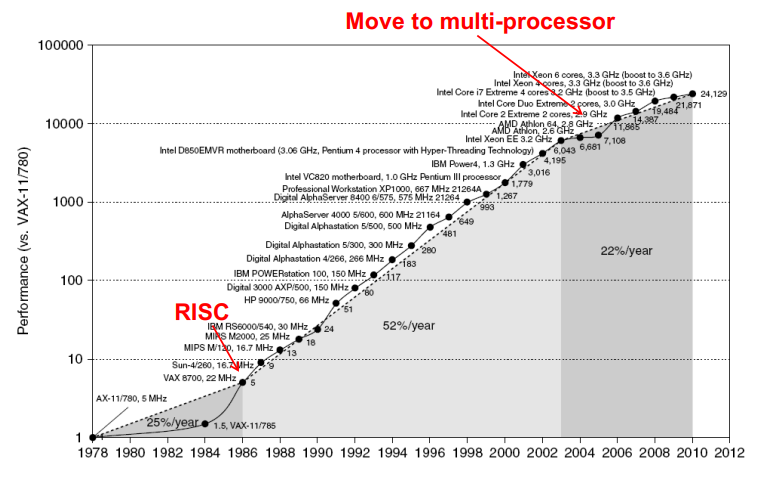
\includegraphics[width=.9\textwidth]{imgs/growth.png}
\caption{Growth in processor performance}
\end{figure}
\noindent
Since 2004, there has been a move from single processors to multiple processors per chip. This was due to two issues with single-processor chips, the maximum power dissipation of air-cooled chips and the lock of more instruction-level parallelism for efficiency. The change has promted a switch from the the old \textbf{Instruction-level parallelism (ILP)} to new models difference models:
\begin{description}
\item[{Data-level parallelism (DLP)}] Parallelising with GPUs in mind using vector processing to process multiple things at once
\end{description}

\begin{description}
\item[{Thread-level parallelism (TLP)}] A focus on multicore concurrency
\end{description}

\begin{description}
\item[{Request-level parallelism (RLP)}] Concurrent processing of multiple requests on a system
\end{description}
\noindent
Many of these require explicit resturcturing of the application to exploit the parallelism. Sometimes this is easy, however in many cases it is quite difficult.
\section{Memory}
Programmers often want unlimited amounts of low latency memory, however, fast memory technology is often much more expensive per bit than slower memory. Fast memory is more expensive as it is both more expensive to produce and is more expensive in terms of energy. An economical solution to this problem is a \textbf{memory hierarchy} which takes advantage of locality and cost-performance of memory technologies. A memory hierarchy is organised into many levels, each level being smaller, faster and more expensive per byte. In almost all cases, all data in one level are also found in the level below, and all data in the lower level are also found in the level below that until the bottom. This is called the \textbf{inclusion property}.
\n
Each level effectively maps addresses from a slower, larger memory to a smaller, faster memory to given the illusion of a large, fast memory being presented to the processor. As we move further away from the processor, the memory in the level below becomes slower and larger.
\begin{figure}[H]
\centering
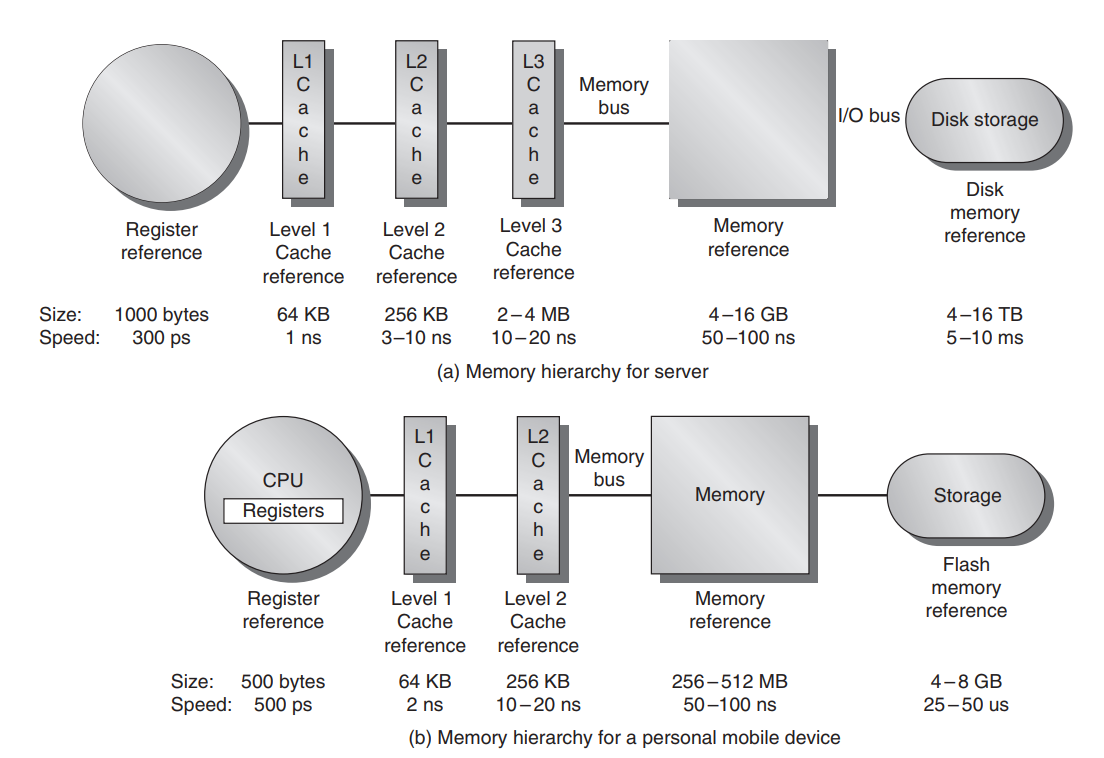
\includegraphics[width=0.9\textwidth, keepaspectratio]{imgs/memory-hierarchy.png}
\caption{The levels in a typical memory hierarchy in a server computer (a) and in a personal mobile device (b).}
\end{figure}
\noindent
Memory hierarchy design becomes even more important now with multicore processors as the aggregate peak bandwidth grows with the number of cores in the processor. Having more processors means a higher memory demand. This is done by multiporting and pipelining caches, use of multiple levels of caches per core, for example using first and/or second level caches per core with a shared third-level cache. In contrast, DRAM's peak bandwidth is only a small fraction of this.
\n
Another consideration in the design of memory hierarchies is power. Traditionally, metrics such as memory access time (determined by cache access time, miss rate and miss penalty) were the focus of optimising the design. However with a significant amount ($\>30$ MB) of on-chip cache, power consumption and amount of on-chip area the memory takes up becomes a bigger factor in memory hierarchy design. 

\subsection{Memory hierarchy basics}
When a word is not found in the cache, the word must be fetched from a lower level in the hierarchy and placed in the cache before continuing. This is called a \textbf{miss}. The need to fetch the work from a lower level in hierarchy requires a higher latency reference. The lower level can be another cache or main memory. Multiple words are called a \textbf{block} and when a miss occurs, the entire block is fetched from efficiency reasons, mostly to take advantage of \textit{spatial locality}.
\subsubsection{Cache associativity}
A key design decision is where the blocks can be placed in a cache. A popular scheme to use is \textbf{set associativity}, where a set is a group of lines in the cache. Each block is mapped to a set and then the block can be placed anywhere within that set. Finding the block won't be in immediate constant time, as the set has to be searched for the block, increasing the cache hit time, but this allows more flexibility in the cache as more of the cache can be used, decreasing the cache miss rate. The set a block belongs to is chosen according to the address of the data:
\begin{center}
(\textit{Block address}) \textsc{mod} (\textit{Number of sets in cache})
\end{center}
\noindent
Having $n$ blocks per set is called \textit{n-way set associative}. A direct-mapped cache would be 1-way set associative which has just one block per set (each block is always placed in the same location) and a fully assocbiative cache only has one set (each block can be placed in any location of the cache).
\begin{figure}[H]
\centering
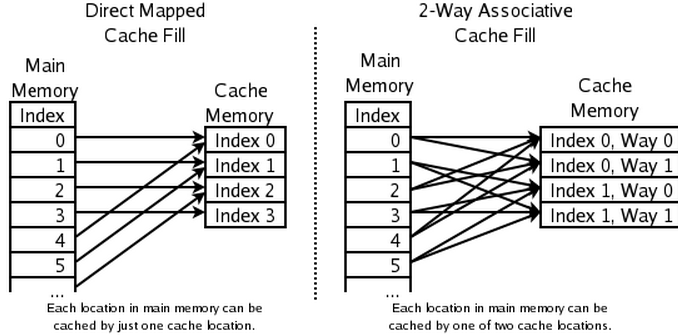
\includegraphics[width=1\textwidth, keepaspectratio]{imgs/cache-associativity.png}
\caption{Cache set associativity}
\end{figure}
\subsubsection{Writing to cache}
Caching date to read is easy as the data in the cache and main memory are identical. However, caching with writing involved is more complications. There are two strategies for writing to cache: \textbf{write-through} and \textbf{write-back}. Both strategies use a write-buffer to allow the cache to make writes asynchronous so as it not have to wait for the time taken to write the data into memory.
\begin{itemize}
\item \textbf{Write-through} cache updates the block in cache and immediately writes through to update lower levels of hierarchy and main memory.
\item \textbf{Write-back} only updates the copy in the cache. Only when the block gets evicted does it write the changes back to lower levels of hierarchy and memory. 
\end{itemize}
\subsubsection{Cache misses}
An important metric to consider when looking at cache is the \textbf{miss rate}. This is the fraction of cache accesses that result in a miss, in other words:
\begin{equation*}
\frac{\textit{Number of cache accesses that miss}}{\textit{Number of cache accesses}}
\end{equation*}
There are three simple categories for cache misses:
\begin{itemize}
\item \textbf{Compulsory} - This is a miss from the first time a block is reference. It is not possible for the block to be in the cache on the first access, so it is a miss and the block has to be brought into the cache. Compulsory misses are cache misses that would occur even with an infinite sized cache.
\item \textbf{Capacity} - If the cache is full and a block is evicted which is later needed again, it is a capacity miss. This typically happens if the cache is not big enough to fit all blocks needed during the execution of a block of code or a program.
\item \textbf{Conflict} - Similar to a capacity miss, except rather than the entire cache being out of space, this miss occurs when the cache is not fully associative and a block is discarded due to the same set of cache lines being full. In other words, the program makes repeated references to multiple addresses from different blocks that map to the same location in cache. This is especially a problem for direct-mapped caches.
\end{itemize}
Note that speculative and multithreaded processors may execute other instructions during a miss to reduce the performance impact of cache misses. However multiple cores add complications, increasing potential for cache misses and adding a fourth \textbf{coherency miss} due to keeping cache in sync across multiple cores.
\n
Ultimately, the miss rate is not always the best metric for determining cache performance. The main issue is it doesn't factor in the cost of a miss, so a better measure is the \textit{average memory access time}:
\begin{equation*}
\text{Average memory access time} = \text{Hit time} + \text{Miss rate} \times\ \text{Miss penalty}
\end{equation*}
\noindent
The \textit{hit time} is the time to hit in the cache (search through the set to find the block) and the \textit{miss penalty} is the time needed to replace the block from memory. 
\subsubsection{Cache and clock rate}
The cache and CPU clock rate are independent, but the speed of memory is important for the clock rate performance of the processor. If memory access time takes two clock cycles instead of one, it is a 100\% increase.
\subsubsection{Six basic cache optimisations}
There are always trade-offs in cache design decisions. Usually they involve decreasing misses, miss penalties and hit times at a cost of the other or at cost of higher power, more space/cost in terms of transistors on the CPU. 
\begin{enumerate}
\item \textbf{Larger block sizes to reduce miss rate} - Increases the block sizes takes more advantage of spatial locality, as more words are moved into the cache with the same block. This reduces compulsory misses but increases capacity and conflict misses due to there being less blocks able to fit in the cache. This also increases the miss penalty because there is more data in the block to write in and out on each miss. 
\n
Choosing a block size depends on both the latency and bandwidth of the memory. High latency and high bandwidth encourage large block size as the miss penalty is smaller due to high bandwidth and more bytes will be written in cache per miss which helps the issue of high latency. Conversely, low latency and low bandwidth would prefer smaller block sizes as the miss penalty is much greater from the low bandwidth, and we do not mind having more misses as the latency is low. 
\item \textbf{Bigger caches to reduce miss rate} - Having a larger total cache size reduces capacity misses. The obvious disadvantage is a longer hit time (more blocks to search through) and increased cost/power consumption as the cache is larger. 
\item \textbf{Higher associativity to reduce miss rate} - Increasing the associativity reduces conflict misses but comes at a cost of higher hit time as there are more blocks to search through per set. 
\item \textbf{More number of cache levels to reduce miss penalty} - It is a difficult trade-off to decide between making the cache fast to keep pace with the CPU clock rate, or to make a cache large to reduce misses and reduce the gap between the processor accesses and main memory accesses. Additional levels of cache can be added in between the processor cache and main memory to simplify the decision. The first-level cache can be kept fast to keep up with the processor while the second/third-level cache is larger to capture accesses that otherwise would have to go back to main memory. Higher level caches focus on misses and so lead to larger blocks, bigger capacity and higher associativity. 
\item \textbf{Giving priority to read misses over writes to reduce miss penalty} - Write buffers create hazards because they hold updated values of data that will be needed on a read miss (a read-after-write) hazard. A solution is to check the write buffer on a read miss. If there are no conflicts, sending the read before the writes reduces the miss penalty as the processor is probably waiting for the read and doesn't have to wait for the write buffer to empty before servicing the read.
\item \textbf{Avoiding address translation during indexing of the cache to reduce hit time} - Caches have to deal with translation from virtual addresses from the processor to a physical address to access memory. By using a page offset (a part of the address identical in both virtual and physical addresses) to index the cache and reduce the hit time as the translation lookaside buffer is no longer needed. 
\end{enumerate}
\subsection{Ten Advanced Optimisations of Cache Performance}
There are five metrics used for cache optimisation. \textit{Hit time}, \textit{miss rate} and \textit{miss penalty} for the memory access time and \textit{cache bandwidth} and \textit{power consumption} given recent trends in architecture design. The ten advanced cache optimisations can be categorised based on these give metrics:
\begin{itemize}
\item \textbf{Reducing the hit time} - Small and simple first-level caches and way-prediction. These optimisations also generally decrease power consumption.
\item \textbf{Reducing the miss penalty} - Critical word first and merging write buffers. These optimisations have little impact on power consumption.
\item \textbf{Reducing the miss rate} - Compiler optimisations. Improvements at compile time means improvements to power consumption. 
\item \textbf{Increasing the cache bandwidth} - Pipelined caches, multibanked caches and non-blocking caches. These techniques result in varying impacts on power consumption. 
\item \textbf{Reducing the miss penalty or miss rate via parallelism} - Prefetching. This generally increases power consumption, especially due to prefetched data that goes unused.
\end{itemize}
Generally these optimisations require additional hardware complexity and sophisticated compiler techniques. 

\subsubsection{Optimisation 1: Small and simple first level caches}
Because of the need to have a fast clock cycle and power limitations for the first-level cache, keeping this cache small and simple help to reduce hit time and power and encourages a limited size. Similarly, this also encourages using lower levels of associativity to reduce hit time and power although this involves more complex trade-offs with the miss rate. Lower associativity reduces power because there are fewer cache lines that need to be accessed.
\n
The \textbf{critical timing path} in a cache hit is a three-step process:
\begin{enumerate}
\item Address the tag memory using the index portion of the address
\item Compare the read tag value to the address
\item Selecting the correct set if the cache is set associative. 
\end{enumerate}
\begin{figure}[H]
\centering
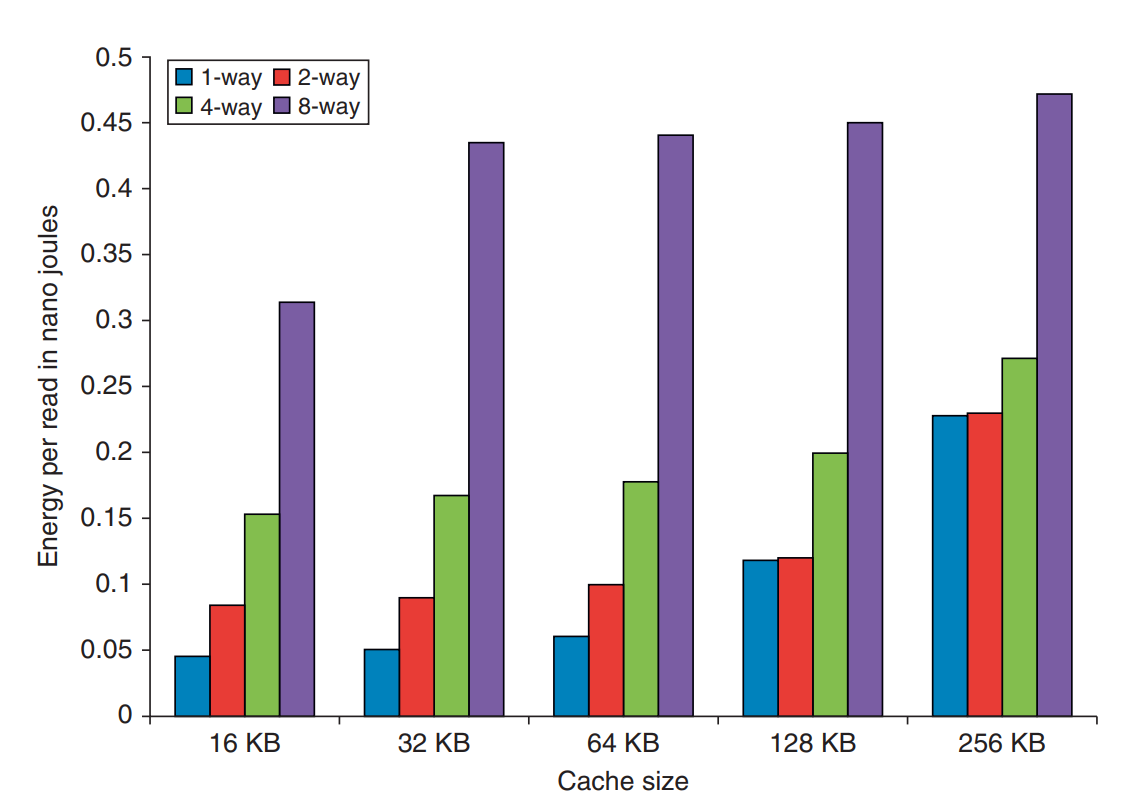
\includegraphics[width=0.9\textwidth, keepaspectratio]{imgs/cache-optimisation1.png}
\caption{Energy consumption per read increases as cache size and associativity increases.}
\end{figure}
Direct-mapped caches can overlap the tag comparison with the transmission of the data to reduce hit time. Because of the clock rate issue arising for larger L1 cache, it may make more sense to increase the associativity rather than the actual cache capacity. More associativity also helps reduce conflict misses, which become more frequent in multi-core processors.

\subsubsection{Optimisation 2: Way prediction}
This is an approach to reduce conflict misses while maintaining high hit speed for direct-mapped cache (no set associativity). For this approach, extra bits are stored in the cache to predict the ``way" - block within the set - of \textit{next} cache access. This means predicting which block within the set is likely to be accessed next and so does not require searching through the set and checking the tag on each block. To do this, the multiplexor is set early to the desired block and only one tag comparison is performed on that clock cycle in parallel while reading the cache data. This is essentially predicting the \textit{way} the multiplexor will select the next block and is not exactly the same as actually predicting what the next block is going to be. Way prediction only predicts the way to pre-set the multiplexor so we potentially only have to do one comparison rather than many comparisons.
\n
An extension to this optimisation is to \textit{actually} predict which block will be used next. This reduces power consumption by using the way prediction to decide which cache block to actually access. This is called \textbf{way selection} and saves power if the prediction is correct but adds significant time on mispredictions as both the access and tag matching must be repeated.

\subsubsection{Optimisation 3: Pipelining cache}
The idea here is to simply pipeline the cache access to improve bandwidth and allow the effective latency of first-level cache to be multiple clock cycles. This will give fast clock cycle time but slow hits. However, this change increases the number of pipeline stages in the processor, which leads to a greater penalty on mispredicted branches, but makes it easier to increase associativity. 

\subsubsection{Optimisation 4: Non-blocking caches}
For pipelined computers that allow out-of-order execution, the processor can continue to fetch instructions while waiting for the data cache to return missing data on a cache miss. A \textbf{non-blocking cache} increases the benefits of this strategy by allowing the data cache to continue supplying cache hits even after a miss. This is essentially a \textit{hit under miss} which reduces the effective miss penalty as the cache is still being used during a miss, rather than be blocked until the previous miss is written. 
\n
An extra, subtle optimisation is to allow hits under \textit{multiple misses}. This further lowers the effective miss penalty but only works if the memory system can service multiple misses (L2 cache must support this).
\n
In general, processors can hide the miss penalty of L1 cache that hits the L2 cache but not miss penalties of L2 cache and above. 

\subsubsection{Optimisation 5: Victim cache}
A \textbf{victim cache} is a small fully associative cache that sits next to the larger cache it is part of. On a cache miss, instead of going lower down the hierarchy, the victim cache is first checked and the block contents swapped. This is like a small cache for the cache to prevent the need to have to go to a lower level in hierarchy and is good if there are many conflict or capacity misses. In particular, this approach is used with direct-mapped cache where conflict misses may occur more frequently. 

\subsubsection{Multibanked caches}
The cache can be split up into independent banks rather than being treated as one monolithic block. This allows simultaneous accesses to different blocks in the cache. 
\begin{figure}
\centering
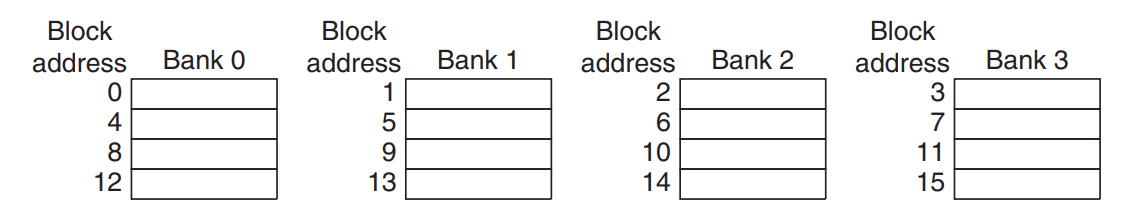
\includegraphics[width=1\textwidth, keepaspectratio]{imgs/multibanked-cache.png}
\caption{Four-way interleaved cache banks using block addressing.}
\end{figure}

\subsubsection{Critical word first and early restart}
This approach has to do with the processor needing only one work of a block at a time. So instead, we don't want to be waiting for the block to be fully loaded before sending the requested word and restarting the processor.
\begin{itemize}
\item \textbf{Critical word first} - Request the missing word first from memory and send it to the processor as soon as it arrives to allow the processor to continue execution before the rest of the words are filled in the block.
\item \textbf{Early restart} - Fetch the words as normal but send the missing word as soon as it arrives in the block. 
\end{itemize} 
The effectiveness of these strategies depends on the block size and likelihood of another access to the portion of the block that has not yet been fetched. With a small cache block size, it is not really worth it to use these strategies as it does not take much more time to write the whole block before returning the word to the processor. Likewise if the likelihood of another access to the same block is high, such as given spatial locality, the effective miss penalty is the non-overlapped time from the reference until the second word arrives.

\subsubsection{Merging write buffer}
Write-through caches need write buffers to be sent to the next lower level of the hierarchy. Even write-back caches need a simple buffer when a block is replaced. If the write buffer contains modified blocks, the addresses can be checked to see if the address of the new data matches the address of a valid write buffer entry. If it does, the new data can be combined with the entry. In other words when storing to a block that is already pending in the write buffer, update the buffer.
\n 
This reduces stalls due to a full write buffer.

\subsubsection{Compiler Optimisations}
This technique does not require any changes to hardware unlike all the previous techniques. The techniques here come from optimising the software where the compiler checks at compile time for optimisations that could improve performance. 

\subsubsection*{Loop Interchange}
Sometimes a program's loops are nested in a non-sequential order such that it does not take advantage of the spatial locality of the way the data is stored. By simply swapping the nesting of the loops, the code can access the data in the order which they are stored in. Assuming that the whole data could not be fit into the cache, this reduces misses from improving spatial locality.
\begin{center}
  \begin{lstlisting}[caption={Loop interchange}, captionpos=b]
    /* Before */
    for (j = 0; j < 100; j++) {
      for (i = 0; i < 5000; i++) {
        x[i][j] = 2 * x[i][j];
      }
    }

    /* After */
    for (i = 0; i < 5000; i++) {
      for (j = 0; j < 100; j++) {
        x[i][j] = 2 * x[i][j];
      }
    }
  \end{lstlisting}
\end{center}
For example if an two-dimensional array of size [5000,100] was allocated such that arr[i,j] and arr[i,j+1] are adjacent in memory then the code above shows how this can be optimised. In the first block, the code would go through the memory in strides of 100 words while the optimised version would access each word sequentially. The latter improves cache performance thanks to locality without affecting the number of instructions created.

\subsubsection*{Blocking}
When having to deal with multiple arrays, with some arrays accessed by rows and others by columns, simply doing loop interchange is not enough as both rows and columns are used in each iteration of the loop. Rather than operate on rows and columns of an array, \textbf{blocking} operates on submatrices or \textit{blocks}.
\begin{figure}[H]
  \centering
  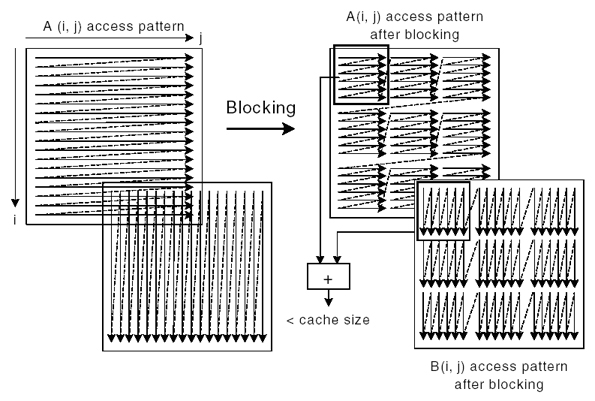
\includegraphics[width=1\textwidth, keepaspectratio]{imgs/cache-blocking.jpg}
  \caption{Example of accessing a 2D array with blocking rather than by row/columns.}
\end{figure}
\noindent
The goal is to maximum memory accesses to the data loaded in the cache before it gets replaced. This can be when multiple matrices are used, so they cannot all fit in the cache and a large number of capacity misses may occur depending on how the each matrix must be accessed. To ensure the elements being accessed can fit in the cache, the matrices are subdivided into blocks. 

\subsubsection{Hardware prefetching}
This technique is to fetch two blocks into cache on a miss instead of just one. The idea is that the next sequential block is also likely to be used in the near future so it is \textbf{prefetched} only with the missing block. This reduces the miss penalty and miss rate as the next block that would otherwise be missed is not. However, the affect can be negative if the next block fetched is unused.
\n
Prefetching relies on utilising memory bandwidth that otherwise would be unused, but if it interferes with other misses it can lower performance as it is doing extra work that doesn't always pay off. If prefetching works, it has a negligible affect on power. However, if it fails it has a very negative impact of power as the hardware has done the extra work of fetching another data block that goes unused.

\subsubsection{Compiler prefetching}
Alternatively to having the hardware do the prefetching, the compiler can insert prefetch instructions to put data in the cache before the processor knows it needs it. There are two types of compiler prefetching:
\begin{itemize}
\item \textbf{Register prefetch} to load the value into a register.
\item \textbf{Cache prefetch} to load data only into the cache and not the register.
\end{itemize}
\noindent
A programmer can manually insert prefetch instructions in code by calling assembly instructions to load data before it is used. However this has many issues as the programmer does not have knowledge of the underlying architecture which the code runs on. The compiler may optimise the prefetch instructions away and different architectures may react to the manual prefetching different.
\n
A \textbf{non-faulting} prefetch means the prefetch instruction does not cause any exceptions and simply turns into no-ops if an exception would occur. Prefetching is only effective if the processor remains unaffected. In other words, the cache should not stall the processor when completeing prefetch instructions. As such, the data caches should be non-blocking. Remember that issuing prefetch instructions are an overhead and the compiler must ensure that the overhead of these instructions do not exceed the benefits.
\n
Loops are good targets for prefetching. If the miss penalty is low, the compiler can just unroll the loop once or twice and prefetch with the execution. If the miss penalty is larger, it uses software pipelining or unrolls many times to prefetch data for future iterations. The idea of \textbf{loop unrolling} is taking the body of the loop and reducing the number of iterations by doing the instructions multiple times in the body. This is to reduce the need for the comparison at the beginning of the loop and leads to a larger binary being produced.
\begin{lstlisting}[caption={Loop unrolling}, captionpos=b]
/* Before */
for (int i = 0; i < 10; i++) {
  delete(i);
}


/* After */
for (int i = 0; i < 10; i+=2) {
  delete(i)
  delete(i + 1)
}
\end{lstlisting}
\noindent
The big advantage of this is the removing of branching conditions at the beginning of each iteration which helps CPU pipelining. The disadvantage is the increased size of the loop body. Too much unrolling may cause the body to no longer fit in the cache which would negative affect performance.

\subsubsection{Optimisation summary}
In summary, the many optimisations focus on improving hit time, bandwidth, miss rate and miss penalty. Each optimisation generally affects other components as well as increasing the complexity of the memory hierarchy. Generally, no technique helps more than one category.
\begin{figure}[H]
  \centering
  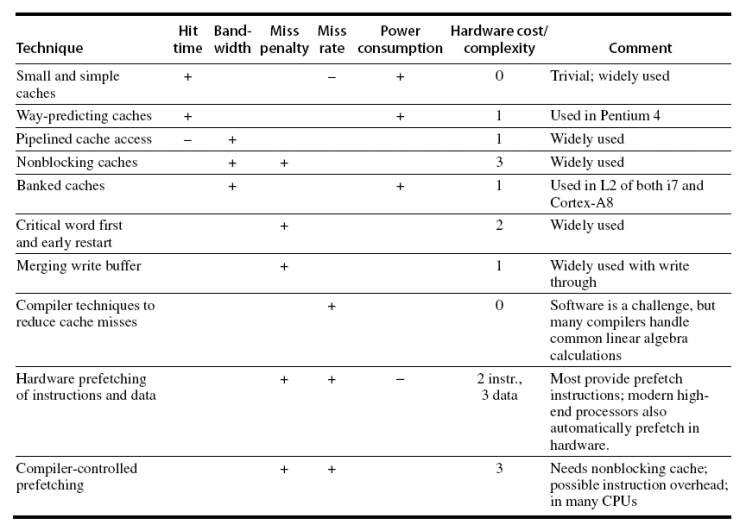
\includegraphics[width=1\textwidth, keepaspectratio]{imgs/cache-optimisation-summary.png}
  \caption{Summary of the ten advanced cache optimisations.}
\end{figure}

\subsection{Memory technologies}
Main memory (commonly known as RAM) is the next level after cache in the memory hierarchy. Main memory cares about both latency and bandwidth as it has to interface between the cache and any I/O. Latency is the primary concern for cache as it affects the miss penalty while bandwidth is the primary concern for multiprocessors and I/O. Although caches benefit more from improvements in latency, it is often easier to improve memory bandwidth. Having multi-level caches and larger block sizes make main memory bandwidth important to caches as well. Often cache designers choose to have larger block sizes to take advantage of high memory bandwidth.
\n
Memory latency uses two measures:
\begin{itemize}
\item \textbf{Access time} is the time between when a read is requested and the desired word arrives.
\item \textbf{Cycle time} is the minimum time between unrelated requests to memory.
\end{itemize}
\noindent
Amdahl suggested that memory capacity should grow linearly with processor speed to keep a balanced system. Unfortunately, the performance of DRAM grows at a much slower pace compared to that of processors. 
\subsubsection{SRAM technology}
SRAM stands for \textit{static} RAM. SRAMs don't need to refresh like DRAMs, so the access time is very close to the cycle time. They typically use more transistors per bit to prevent information from having errors when read. It also needs only minimal power to retain the charge to retain all the bits. These days all levels of cache using SRAM and are integrated with the processor chip.

\subsubsection{DRAM technology}
The \textit{D} is DRAM stands for \textit{dynamic}. To be able to put more bits in per chip, DRAMs only use a single transistor to store each bit. Reading that bit will destroy the information, which is why the DRAM cycle time is traditionally longer than the access time, as the information must be re-written after each read. Recent DRAM technologies introduce multiple banks to allow the rewrite portion of the cycle to be hidden. Additionally, because each bit is only stored on one transistor, the bits must be periodically \textit{refreshed}. This requirement means that the memory is occasionally unavailable while it is refreshing. The time for a refresh is typically a full memory access for each row of the DRAM. 
\n
DRAM address lines are multiplexed. One-half of the address is sent first during \textbf{row access strobe} (RAS) and the other half of the address is sent during \textbf{column access strobe} (CAS) afterwards.

\subsubsection{Memory optimisations}
Due to the pressure of memory performance having to keep up with the processor-memory gap, many small optimisations have been made to DRAM. Generally, this has led to increased bandwidth, sometimes at the cost of higher latency.
\begin{itemize}
\item DRAMs have timing signals that allow repeated access to the row bugger without required another row access time. This allows multiple access to the same row without increased latency
\item A clock signal was added to the DRAM interface so that DRAM becomes \textbf{synchronous}. An asynchronous would require overhead to synchronise with the memory controller on every transfer. SDRAMs have a programmable register to hold the number of bytes requested to send many bytes over several cycles per request. In burst mode, DRAM supports critical word first transfers.
\item A wider interface was added to allow a wider stream of bits to be taken from the memory without making the memory system too large. While they initially offered 4-bit transfers, newer technologies like DDR3 have up to 16-bit buses.
\item A major DRAM innovation to increase bandwidth is to transfer data on both the rising and falling edge of the clock signal to double the peak data rate. This is known as the \textbf{DDR} (double data rate).
\item Multiple banks were introduced on each DRAM device to provide more advantages of interleaving and help with power management. The banks can operate independently. This effectively adds another segment to the address, which now contains bank number, row and column address. However, when an address is sent to a new bank, that bank must be opening, which introduces a delay.
\end{itemize}
\noindent

\subsubsection*{Reducing power in SDRAMs}
Power consumption of DRAM depends on the operating voltage. The additiona of banks in DRAM also reduces the power consumption as only the row in a single bank is read and precharged. Additionally, recent SDRAMs support a \textbf{low power mode}, which tells the DRAM to ignore the block, essentially disabling SDRAM except for the internal automatic refresh. The cost incurred here is delay leaving low power mode.

\subsubsection{Flash memory}
Flash memory is a type of EEPROM (Electronically Erasable Programmable Read-Only Memory), which is normally read-only, but can also be erased. A key property of flash memory is that it can hold its contents \textit{without any power}. There are a few key differences between flash memory and DRAM:
\begin{enumerate}
\item Flash memory must be erased (in blocks) before being over-written.
\item Flash memory is static (non volatile), so it draws significantly less power when not reading and writing.
\item Flash memory has a limited number of write cycles for any block. Uniform distribution of writes will help to maximise the lifetime of a flash memory system.
\item Flash memory is cheaper than SDRAM but more expensive than disks.
\item Flash memory is slower than SDRAM but faster than disk. 
\end{enumerate}
Advancements in flash memory technology have made it viable for some memory hierarchies, especially in mobile devices where battery life is important. It also serves as a solid-state replacement for disks.

\subsubsection{Memory dependability}
An issue with error in memory comes from cosmic rays striking a memory cell. These dynamic errors, called \textbf{soft errors} are changes to thce cell contents, but not the circuitry. These errors can be detected and fixed by error correcting codes. Memory manufactured often come with spare rows to replace defective ones. \textbf{Hard errors} are permanent changes in the operation of one or more memory cells, which can occur during operation. The spare rows are used to mitigate this problem.
\n
A solution called \textbf{Chipkill} was introduced by IBM. It is a RAID-like error recovery technique for memory to detect and recover from errors.

\subsection{Virtual memory and virtual machines}
Program memory must be protected from other processes which can steal or change memory directly otherwise. This can be accomplished both via virtual memory and virtual machines.

\subsubsection{Protection via virtual memory}
Virtual memory is used to keep processes in their own memory space and prevent processes looking and writing into another process's memory. Page-based virtual memory, including the translation lookaside buffer is the main mechanism to protect processes from each other. The operating system and architecture must work together to allow processes to share hardware yet not interfere with each other. To do this, the architecture has to limit what a process can access while running while allow the operating system more access. The role of the architecture is as follows:
\begin{itemize}
\item \textbf{Provide user mode and supervisor mode} to indicate whether a user process is running or an operating system process.
\item \textbf{Protect aspects of CPU state} so a user process can use but no write. This typically involves a user/supervisor bit. Users are prevented from writing to this state, otherwise the operating system cannot control user processes which give themselves supervisor privileges and disable memory protection.
\item \textbf{Provide mechanisms for switching between user and supervisor mode} - This is typically done with system calls, where the user process transfers control to a dedication supervisor code space. The return to user mode is like a subroutine return that restores the previous process space.
\item \textbf{Provide mechanisms to limit memory access} - This protects memory state of a processing without having to swap for a context switch all the time.
\item \textbf{Provide TLB to translate addresses} - The TLB translates between virtual memory addresses and physical addresses. Requiring one memory access to obtain the physical address and another to get the data is far too costly. The solution is a cache of address translations so a memory access rarely required a second access to translate the address. 
\end{itemize}

\subsubsection{Protection via virtual machines}
Virtual machines support isolation and security. They provide a complete system-level environment at the ISA level and allows different ISAs and operating system to be presented to user programs. The fotware the supports VMs is the \textbf{virtual machine monitor} (VMM) which determines how to map virtual resources to physical resources. There is a high cost for virtualisation workload, but this is enabled thanks to the raw speed of processors, making the overhead acceptable.
\n
To virtualise a processor, the VMM must control almost everything. It adds a level of memory between the physical and virtual memory and maintains a shadow page table that maps guest virtual address to physical addresses.

\section{ILP - Instruction Level Parallelism}
Since about 1985, pipelining has been used to overlap the execution of instructions so that instructions can be evaluated in parallel and improve performance. This overlap is called \textbf{instruction-level parallelism} (ILP).
\n
There are two main approaches to exploiting ILP:
\begin{enumerate}
\item \textbf{Hardware based dynamic approaches} - These approaches rely on hardware to help discover and exploit parallelism dynamically. Processors which use the dynamic approach dominate the desktop and server markets. However, these approaches are not used much in embedded processors on mobile devices where energy efficiency is of more importance. 
\item \textbf{Compiler based static approaches} - These approaches use software technology to find parallelism statically at compile time. This is done more for mobile devices but often are not as successful outside of scientific applications.
\end{enumerate}
\noindent
When exploiting instruction-level parallelism, the goal is to minimise CPI (cycles per instruction). The value of the CPI is the sum of the base CPI and all contributions from stalls.
\begin{align*}
  \text{Pipeline CPI} & = \text{Ideal pipeline CPI} \\
                      & + \text{Structural stalls} \\
                      & + \text{Data hazard stalls} \\
                      & + \text{Control stalls}
\end{align*}
\noindent
The \textbf{ideal pipeline CPI} is a measure of the maximum performance attainable by the implementation. We aim to reduce the time taken by each of the stalls to decrease overall CPI, or in other words, increase the instructions per cycle.
\begin{figure}[H]
  \centering
  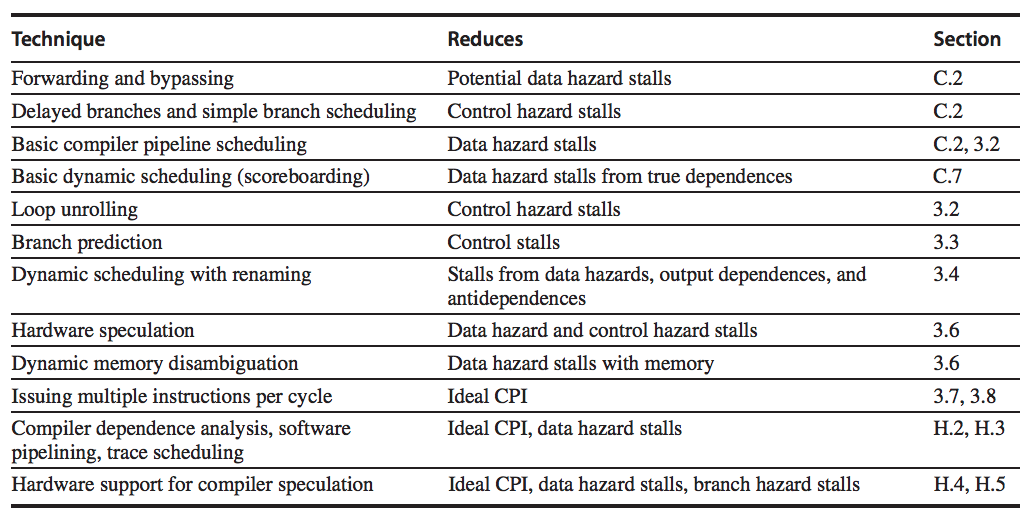
\includegraphics[width=1\textwidth, keepaspectratio]{imgs/ilp-techniques.png}
  \caption{Major ILP techniques and their effects}
\end{figure}
\noindent
The amount of parallelism avaiable within a \textbf{basic block} - A single line of code sequence with no branches in except to the entry and no branches out except at the exit - is pretty small. Since the instructions in a basic block are likely going to depend on each other, the amount of overlap that can be exploited is going to be less than the average basic block size. To get substantial performance increase, we must exploit ILP \textit{across multiple basic blocks}.
\n
A common way to increase ILP is to exploit parallelism in loop iterations. This is called \textbf{loop-level parallelism}. For example, here is a loop that adds two arrays and is completely parallel:
\begin{lstlisting}[caption={Example of parallel loop}, captionpos=b]
for (i = 0; i < 1000; i++) {
  x[i] = x[i] + y[i];
}
\end{lstlisting}
\noindent
Every iteration of the loop can overlap with any other iteration, but there is no opportunity to overlap within each iteration. Basic techniques such as unrolling the loop statically or dynamically as discussed earlier can work to increase parallelism. An important alternative to exploit loop-level parallelism is the use of SIMD (Single instruction, multiple data) in vector processors and GPUs. A SIMD instruction exploits data-level parallelism by operating on a number of data items in parallel (typically 2 to 8). A vector instruction can exploit data-level parallelism by operating on many data items in parallel using both parallel execution units and a deeper pipeline.

\subsection{Dependencies}
Finding out how one instruction depends on another is critical to determining how much parallelism exists in a program and how that parallelism can be exploited. In particular, we have to determine which instructions can run in parallel. Two instructions are parallel if they can execute simultaneously in a pipeline of arbitrary depth without casuing any stalls. The key then is to determine whether an instruction is dependent on another instruction.
\n
There are three different types of dependencies:
\begin{enumerate}
\item Data dependences (also called true data dependences)
\item Name dependences
\item Control dependences
\end{enumerate}
\noindent
An instruction $i$ is \textit{data dependent} on instruction $j$ if either:
\begin{itemize}
\item Instruction $j$ produces a result that may be used by instruction $i$
\item Instruction $i$ is data dependent on instruction $k$, and instruction $k$ is data dependent on instruction $j$
\end{itemize}
Any dependent instructions cannot be executed simultaneously. 

\subsubsection{Data Dependences (True data dependency)}
Data dependences are a property of programs. Essentially, it is waiting for the output of another instruction to take in data for this instruction's input. The pipeline organisation determines if a dependence is detected and if it causes a stall. A \textbf{data hazard} is what happens as a result of a dependency. The difference is important to understanding how instruction-level parallelism can be exploited.
\n
The presence of a data dependence conveys the following:
\begin{itemize}
\item The possibility of a hazard
\item The order in which results must be calculated
\item An upper bound on how much parallelism can be possibly exploited in ILP.
\end{itemize}
\noindent
Because a data dependence limits the amount of ILP expolitation, it has to be overcome if possible. There are two different ways about this:
\begin{enumerate}
\item Maintaining the dependence but avoid the hazard
\item Eliminating the dependence by transforming the code
\end{enumerate}
Dependencies that flow through memory locations are often difficult to detect. because two addresses may refer to the same location but look different.

\subsubsection{Name Dependences}
Name dependencies occur when two instructions use the same register or memory location. There is no actual flow of data between the instructions assoicated with the names. As such this is not a true data dependence, but it is a problem when re-ordering instructions. There are two types of name dependences between an instruction $i$ that comes before instruction $j$ in the program order:
\begin{enumerate}
\item An \textbf{anti-dependence} between instruction $i$ and $j$ occurs when instruction $j$ writes a register or memory location that instruction $i$ reads (A write after read dependence). The original order is important to ensure the $i$ reads the correct value.
\item An \textbf{output dependence} happens when instruction $i$ and $j$ write to the same register or memory location. The ordering must be preserved to make sure the final value written corresponds to the value from instruction $j$.
\end{enumerate}
\noindent
These are both name dependenices and unlike true data dependencies, no value is being transmitted between the instructions. Since these name dependences are not a true dependence, instructions involved in a name dependence can execute simultaneously or be re-ordered if the name used in the instructions is changed so the instructions no longer conflict with each other. This is usually done by \textbf{register renaming}. Register renaming can be done either statically by the compiler, or dynamically by the hardware.

\subsubsection{Data Hazards}
A hazard exists whenever there is a name or data dependence between instructions that are close enough that the overlap during execution would change the order of access to the operand involved in the dependence. Because of the dependence, we have to preserve the \textbf{program order} - the order the instructions would execute in if executed sequentially one at a time as determined by the original program. Detecting and avoiding hazards ensures that necessary program order is preserved.
\n
Data hazards may be classified as one of three types, depending on the order of read and write accesses of the instructions. Here are the possible data hazards for two insturctions $i$ and $j$ in that order.
\begin{itemize}
\item \textbf{RAW (read after write)} - When $j$ tries to read a value before $i$ writes to it, so $j$ is getting the \textit{old} value. This is a true data dependence and cannot be executed out of order as $j$ \textit{must} wait for $i$ to write the value before it can read.
\item \textbf{WAW (write after write)} - When $j$ tries to write an operand before it is written by $i$. This causes the write to be performed in the wrong order, leaving the value written by $i$ rather than the value written by $j$ in the destination. This hazard corresponds to an \textit{output dependence} and can be fixed by renaming techniques.
\item \textbf{WAR (write after read)} - When $j$ tries to write to a location before $i$ reads from it, so $i$ incorrectly gets the new value. This is an anti-dependence and again can be solved with renaming techniques. WAR hazards typically occur when there are some instructions that write results early in the instruction pipeline and other instructions read the source later in the pipeline, or if the instructions are re-ordered.
\end{itemize}

\subsubsection{Control Dependences}
A control dependence checks the ordering of instruction $i$ with respect to a branch instruction to make sure that it is only executed in the correct order and only when it should be according to the branch. In general, control dependencies must be preserved to preserve program order. Here is the simplest example of a control dependence:
\begin{lstlisting}[caption={Simple if then statement showing control dependences}, captionpos=b]
if p1 {
  S1;
};

if p2 {
  S2;
};
\end{lstlisting}
\noindent
\texttt{S1} is control dependent on \texttt{p1} and \texttt{S2} is control dependent on \texttt{p2} but not on \texttt{p1}. There are two constraints imposed by control dependences:
\begin{enumerate}
\item An instruction that is control dependent on a branch cannot be moved before the branch so that its execution \textit{is no longer controlled} by the branch. For example, the instruction from the \texttt{then} portion of an if statement cannot be taken and moved before the actual if statement.
\item An instruction that is not control dependent on a branch cannot be moved \texttt{after} the branch so that its execution is controlled by the branch. For example, instructions before an if statement cannot be moved into the \texttt{then} portion inside the if statement.
\end{enumerate}
\noindent
If processors preserve strict program order, they ensure that control dependences are preserved. Sometimes, we may be willing to execute instructions that should not have been executed. Even though this violates control dependencies, this is fine if it can be done without affecting the correctness of the program. In other words, a control dependence is not a critical property that must be preserved. 

\subsection{Compiler techniques}
Compiler techniques are crucial for processors that use static scheduling. These techniques can enhance a processor's ability to exploit ILP.

\subsubsection{Pipeline scheduling}
To keep the pipeline full and working, parallelism between instructions can be exploited by finding sequences of unrelated instructions that can be overlapped in the pipeline. In order to avoid pipeline stalls, execution of dependent instructions must be separated by a distance in clock cycles equal to the pipeline latency of that instruction.
\n
By scheduling overlapping instructions during stalls, the total clock cycles required for executing certain code fragments can be decreased.

\subsubsection{Loop unrolling}
The issue with many loops is there is a high overhead for managing the loop, such as branching instruction at the end of loops. A simple way of increasing the number of instructions relative to loop overheads is \textbf{loop unrolling}. Unrolling replicates the loop body so that more instructions are done each iteration and therefore decrease the number of iterations of the original loop. This can only be done if the instructions of the loop body are \textbf{independent} from each other. 
\n
Loop unrolling can also be used to improve scheduling. Because it eliminates branching, it can allow instructions from different iterations to be scheduled together. Different registers will need to be used to prevent data dependencies for effective scheduling. 
\n
Of course in a real program, sometimes the upper bound of the loop is not known until run time. For example if the  upper bound is $n$ and we would like to unroll the loop to make $k$ copies of the body, we need to generate a par of consecutive loops rather than a single unrolled loop. The first loop executes $(n\ \text{mod}\ k)$ times with the body of the original loop. The second is the unrolled loop body that iterates $\frac{n}{k}$ times. This is similar to a techniques called \textit{strip mining}, which is used in vector processors. If the number of iterations is high, most of the execution time will be spent in the second unrolled loop rather than the first $(n\ \text{mod}\ k)$ loop.
\n
In order to obtain the final unrolled code, all following steps must be done:
\begin{itemize}
\item Determine if loop unrolling is useful by finding if each loop iteration is independent.
\item Use different registers to avoid unnecessary constraints such as name dependences
\item Eliminate extra test and branch instructions and adjust loop termination/iteration code
\item Determine if loads and stores in the unrolled loop can be interchanged by checking the loads and stores from different iterations are independent. This involves checking the memory addresses to see that they do not refer to the same address.
\item Schedule the code and preserve any dependences needed to make sure the behaviour of the code stays the same.
\end{itemize}
\noindent
A limit to the benefits of unrolling is the growth in code size. For larger loops, the increased code size is a concern as it causes increases misses in the instruction cache as the loop may be too big to fit all instructions in a single iteration in the cache.

\subsection{Branch Prediction}
Loop unrolling is a way to reduce the number of branch hazards by reducing the number of branching instructions. Another way to reduce performance loss is to predict how branches will behave. 

\subsubsection{Dealing with branches}
There are a few simple schemes to deal with branching:
\begin{itemize}
\item \textbf{Freeze} or \textbf{flush} the pipeline - This stalls the pipeline until the result of the branch is known. This is very simple, but not efficient as there is a high cost to every branch instruction (loss of parallelism via pipeline). 
\item \textbf{Predict not taken} - By always assuming the branch is not taken, the pipeline can continue to operate as normal when it seems a branching instruction. The cost is having to throw away work if the branch goes the other way and complexity arises from having to \textit{back out} of wrong decisions. 
\item \textbf{Delayed branch} - In this scheme, the execution cycle with a branch delay of 1 is: 
\begin{center}
\texttt{branch instruction}
\\ \texttt{sequential successor${}_{1}$}
\\ \texttt{branch target if taken}
\end{center}
The sequential successor is the \textbf{branch delay slot}. This instruction is executed regardless if the branch is taken or not. 
\end{itemize}

\subsubsection{Static branch prediction}
To improve compile-time branch prediction, profiled information collected from earlier runs can be used. A key observation for this is that the behaviour of branches is usually \textit{bimodally distributed} - that is, an individual branch is often highly biased towards taken or not taken. As such, branches can be predicted statically based on this strategy. 

\subsubsection{Dynamic branch prediction}


\subsection{Dynamic scheduling}
Dynamic scheduling is a method where the hardware rearranges the instruction execution to reduce stalls while maintaining data flow and exception behaviour. 
\n
\textbf{Advantages}:
\begin{itemize}
\item Allows code compiled with one pipeline in mind to run efficiently on a different pipeline so there is no need for multiple binaries or need to recompile for different microarchitectures. 
\item It can handle cases where dependences are not known at compile time. 
\item Allows the processor to tolerate unpredictable delays such as cache misses by executing code while waiting for the miss to resolve. 
\end{itemize}
\noindent
The cost of dynamic scheduling is a substantial increase in hardware complexity.
\n
The idea is to have \textit{out-of-order} execution and \textit{out-of-order} completion. For example, consider the following instructions in order:
\begin{lstlisting}
DIV.D	F0, F2, F4
ADD.D	F10, F0, F8
SUB.D	F12, F8, F14
\end{lstlisting}
\noindent
The \texttt{SUB.D} instruction cannot execute until \texttt{ADD.D} finishes, but \texttt{ADD.D} is data dependent on \texttt{DIV.D}. This creates a performance limitation which can be eliminated with out-of-order execution. To avoid structural hazards, we still use in-order instruction issue, but want instructions to execute as soon as operands are available.
\n
Out-of-order execution introduced the possibility of WAR and WAW hazards, which would normally not exist in a five-stage pipeline. 

\subsubsection{Tomasulo's Algorithm}
In Tomasulo's scheme, register renaming is provided by \textbf{reservation stations}. The basic idea is that a reservation station fetches and buffers an operand as soon as it is available, eliminating the need to get the operand from a register. Additionally, pending instructions will designate which reservation station will provide their input. There are sometimes more reservation stations than real registers, which can even eliminate hazards coming from name dependences. 
\n
Having registration stations leads to two other important properties:
\begin{enumerate}
\item Hazard detection and execution control are distributed - that is to say the information held in the reservation stations at each functional unit determines when an instruction can begin execution at that unit.
\item Results are passed directly to functional units from the reservation stations where they are buffered, rather than going through registers.
\end{enumerate}
\noindent
The algorithm goes through three steps, although each step can take an arbitrary number of clock cycles:
\begin{enumerate}
\item \textbf{Issue} - Get the next instruction from the instruction queue. If there is a matching reservation station that is empty, issue the instruction to the station with the operand values. If there is no empty reservation station then there is a structural hazard and the instruction stalls until the station is free. If the operand values are not available, also stall the instruction. This step renames registers to eliminate WAR and WAW hazards.
\item \textbf{Execute} - When an operand becomes available, place it into any reservation station waiting for it. When all operands are available, the operation can be executed. Independent functional units can all issue instructions simultaneously, although only one ready instruction in a unit will be chosen. 
\n
Load and store instructions use effective addresses to maintain program order. This is to prevent hazards through memory. Additionally, no instruction is allowed to initiate execution until all branches that proceed it in program order have been completed to preserve exception behaviour. 
\item \textbf{Write result} - Once the result is available, write it to the common data bus and from there write into registers and any reservation stations that need this result. Store instructions are buffered in a store buffer until both the value to be stored and the store address is available.
\end{enumerate}

\subsection{Hardware-based speculation}
Although branch prediction can reduce the direct stalls from branches, for a processor to execute multiple instructions per clock, just predicting branches accurately is not enough to get the desired amount of ILP. 
\n
Hardware-based speculation speculates the outcome of a branch and executes the program \textbf{as if} the prediction was correct. It has a subtle difference from branch prediction with dynamic scheduling as the instructions are actually executed. The key idea is to allow instructions to execute out of order, but commit the results \textit{in order} if the prediction was correct. Adding this commit phase requires additional hardware buffers to hold the results of instructions that have finished execution but have not yet been committed. 

\subsubsection{Reorder buffer}
The reorder buffer provides additional registers like how Tomasulo's provides reservation stations. The buffer holds the result of an instruction between completion and commit. Hence, the buffer is a source of operands for instructions just like reservation stations provide operands in Tomasulo's. The difference is that the register file is not updated until the instruction is committed. 
\n
Each entry in the reorder buffer contains four fields:
\begin{itemize}
\item \textbf{Instruction type} - For example branch, store, register
\item \textbf{Destination field} - Supplies the register number or memory address where the result should be written to
\item \textbf{Value field} - Holds the value of the instruction result
\item \textbf{Ready field} - Indicates that the instruction has been executed and the value is ready.
\end{itemize}
\noindent
Recovery in the reorder buffer is done by clearing all entries that appear after the mis-predicted branch. Exceptions are handled by not recognising the exception until it is ready to commit. 

\subsection{Multiple issue and static scheduling}
In order to achieve CPI of less than one, multiple instructions must be executed per clock cycle. There are three different solutions to this:
\begin{enumerate}
\item Statically scheduled superscalar processors
\item VLIW (very long instruction word) processors
\item Dynamically scheduled superscalar processors
\end{enumerate}
The two superscalar processors issue a varying number of instructions per clock, in-order if statically scheduled and out-of-order if dynamically scheduled. The VLIW processor will issue a fixed number of instructions either as one large instruction or as a fixed instruction packet with parallelism among instructions explicitly indicated. 
\begin{figure}[H]
\centering
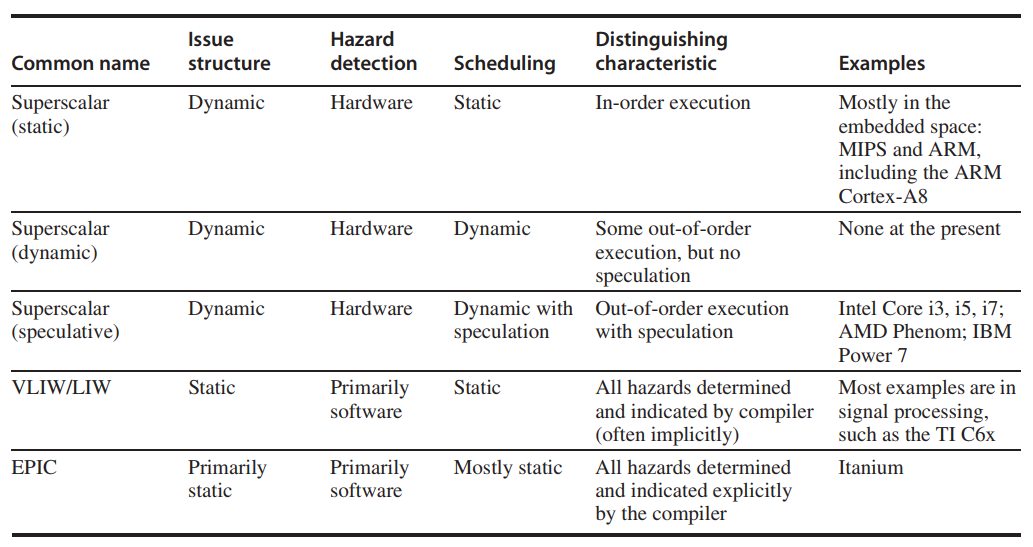
\includegraphics[width=1\textwidth, keepaspectratio]{imgs/multiple-issue.png}
\caption{Summary of five primary approach in use for multiple-issue processors.}
\end{figure}
\noindent
The potential advantage of a multiple-issue processor over a vector processor is the ability to extract parallelism from less structured code and ability to easily cache all forms of data.

\subsubsection{VLIW Processors}
VLIW packages multiple operations into one very long instruction. To keep the functional units busy, there must be enough parallelism in a code sequence to fill the available operation slots. Parallelism can be uncovered by unrolling loops and scheduling the code within the larger loop body. 
\n
There are many issues with the VLIW model:
\begin{itemize}
\item \textbf{Statically finding parallelism} - Parallelism must be discovered statically and laid out in a way to create the very long instruction.
\item \textbf{Increase in code size} due to aggressively unrolling loops to fill functional unit slots.
\item \textbf{Limitations of lockstep operation} - No hazard detection hardware. 
\item \textbf{Binary code compatibility} - 
\end{itemize}

\subsection{Dynamic scheduling, multiple issue and speculation}

\section{Simulation}
The issue with designing architectures is it is \textit{expensive}. These costs involve:
\begin{itemize}
\item Cost of high-level design
\item Cost of verification of design
\item Cost of low-level design
\end{itemize}
If someone designs some new ``trick" for feature, they have to test it to see how well it works. The only economic option is to run it in a \textbf{simulator}.
\n
A simulator could be many things:
\begin{itemize}
\item CPU Simulator - Simulates a CPU by accepting assembly code, processing it and emitting the correct result
\item Microarchitecture simulator - Simulates the underlying microarchitecture (e.g. cache, dynamic instruction translation etc)
\item Full-system simulator - Simulate everything and also deal with IO
\item System-on-chip simulator -CPU + GPU + additional processors + network + IO
\end{itemize}

\subsection{Scope of simulation}
Different levels of simulation exist, some try to simulate everything while others may only simulate the instruction set.
\begin{itemize}
\item \textbf{Full cycle-accurate simulation} - This simulates everything but is a slow approach due to simulating entire CPU accurately being very complicated
\item \textbf{Instruction set simulation} - This is a functional simulation to only simulate the functionality of the CPU, but not simulating exactly how everything works
\item \textbf{Sampling based approach} - Not deterministic and samples differently on every run. The challenge is how to choose what to sample. Phases of the CPU need to be detected to be able to sample all different phases.
\end{itemize}
\noindent
A sampling simulator tries to solve the speed issue of simulators as it only fully simulates a small part of the code running on the simulated platform fully, then run the rest is some other way. 

\subsection{Challenges}
There are many different challenges for a sampling simulation.
\begin{itemize}
\item What to sample
\item IO
\item System calls
\item Resource sharing and context switching
\item Building an accurate statistical model
\item The warming problem
\item Measuring IPC at given intervals
\end{itemize}

\subsubsection{The warming problem}
The warming problem is the idea of how to simulate a CPU that's been ``warmed up" with some instructions with data already in the cache or memory. This is also an issue when a simulator transitions from one type of simulation.
\n
For example, how would we restart cycle-accurate simulation after running in a functional mode and what is the state of the processor? There are a few solutions to this:
\begin{itemize}
\item Simply restart with previous state - This could simulate parts of the processor in the fast forward state, but is slow and inaccurate
\item Live points
\item Reusable warm architectural checkpoints
\item Multiple checkpoints allows simulation parallelism
\end{itemize}

\subsection{Checkpointing}
There are two types of checkpointing:
\begin{itemize}
\item \textbf{High level} - Where cache, directory tags and complete memory data is restored (~10-200MB)
\item \textbf{Low level} - Where registers, TLB, branch predictor, cache tags and touched memory data is restored (~142KB)
\end{itemize}
Both types of checkpointing can be used together. 

\subsection{Accuracy}
It is very difficult to get simulators that are completely accurate and it is also difficult to measure that accuracy. Some simulators are \textit{verified} with formal methods to perform identically (with some tolerance) to hardware. This means they have a certificate from the manufacturer and are generally the most accurate kind of simulator. 
\n
However, modern microprocessors are very complex and nearly impossible to simulate completely accurately. For example a real processor might have bugs that the simulator does not taken into account. Of course the simulator itself can also have bugs. It is important not to fully trust simulation due to accuracy issues, and it is always better to try it on real hardware if the costs permit. A FPGA is an alternative, but only for high level design simulation. 

\section{Programmable Logic}
Programmable logic is very useful as creating Application-specific integrated circuits (ASICs) are very expensive. Programmable logic chips like FPGAs can be mass produced and customised. They may also be faster and more power efficient for parallel tasks. 
\n
Sometimes a general purpose processor is not preferred as it might need an operating system - more to go wrong - or might not have the power or bandwidth. They are also less specialised for particular tasks compared to a programmable device. 
\n
FPGAs are used for hardware prototyping and are a good alternative to simulation. High level design can be generated for a new processor design and flashed onto the FPGA to test it out. Because it is running on some actual hardware, this approach is also much faster than pure simulation. 
\begin{figure}[H]
\centering
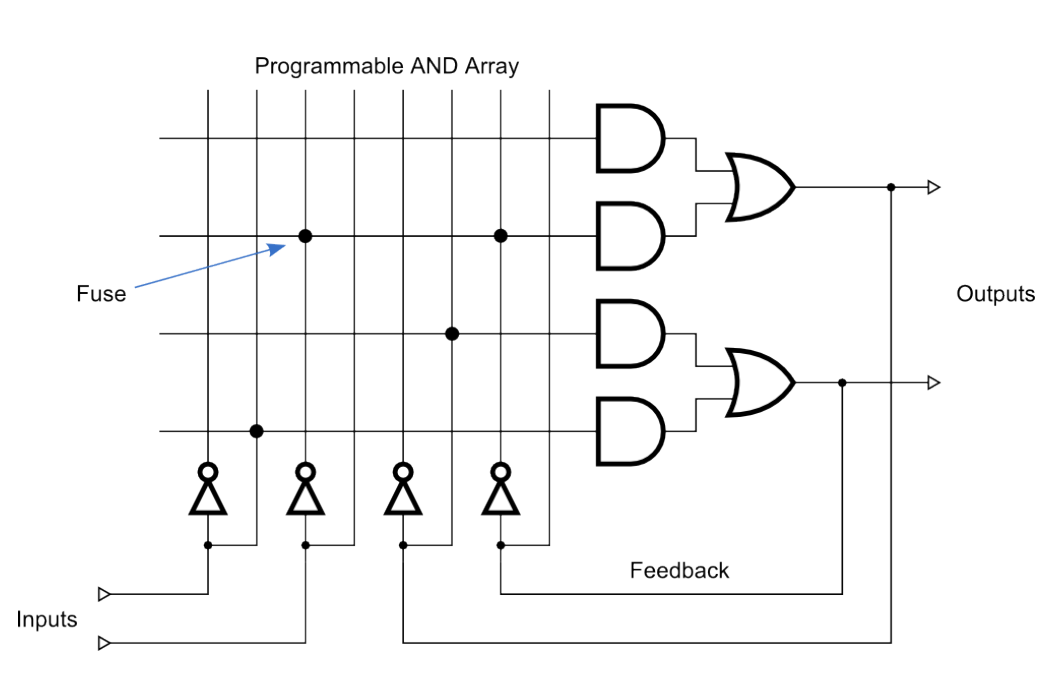
\includegraphics[width=0.9\textwidth, keepaspectratio]{imgs/pld.png}
\caption{Programmable Logic Device}
\end{figure}
\noindent
Original programmable logic devices only had 20-30 logic functions are were ``programmed" by fusing the circuits. More complicated logic devices can be created by connected many PLDs together with a global interconnect matrix (GIM). This leads to two level of programmability and more complex logic functions.
\n
Some PLDs are not reprogrammable, especially if it blows the physical fuses to program the device.

\subsection{FPGA}
A Field Programmable Gate Array (FPGA) has a different architecture compared to PLDs. They contain a mesh of configurable logical blocks (CLBs) which are all connected within a switching matrix. Each \textbf{CLB} performs a logical function such as XOR, AND etc. The switches are then programmed to connect the CLBs to perform more complex logical functions. The IO blocks are on the outside of the FPGA logically to connect to the outside world. These blocks contain special hardware to allow analogue communication, delay circuitry and voltage regulation. 
\begin{figure}[H]
\centering
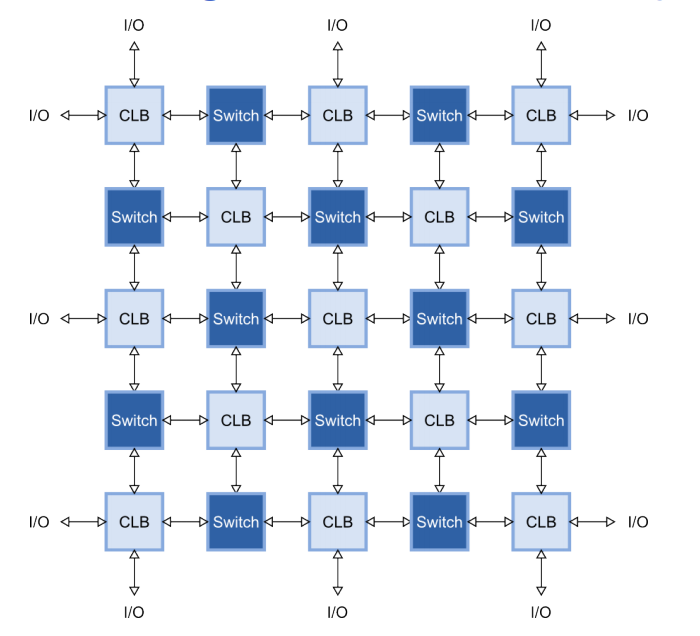
\includegraphics[width=1\textwidth, keepaspectratio]{imgs/fpga.png}
\caption{A FPGA}
\end{figure}
\noindent
Switches are flashed once for good and cannot be changed. These \textbf{fuses} or \textbf{antifuses} define the switching network and logical units. This is useful for significantly less wire delay, less hardware and no need for loading or static storage of the bitstream. 
\n
The circuits can be reconfigured by loading a \textbf{bitmap} or \textbf{bitstream} which defines which connections are open or closed and the look up tables (LUTs) of the CLBs. This allows an FPGA to be re-configurable at any time, though it usually times some time to change the configuration. 
\n
\textbf{CLBs} are implemented using lookup tables with the bits set to define the logic function. For example in figure \ref{fig:clb}, the bits are mapped to define an AND function. The output is stored in a \textbf{flipflop} or used as input to another lookup table. 
\begin{figure}[H]
\centering
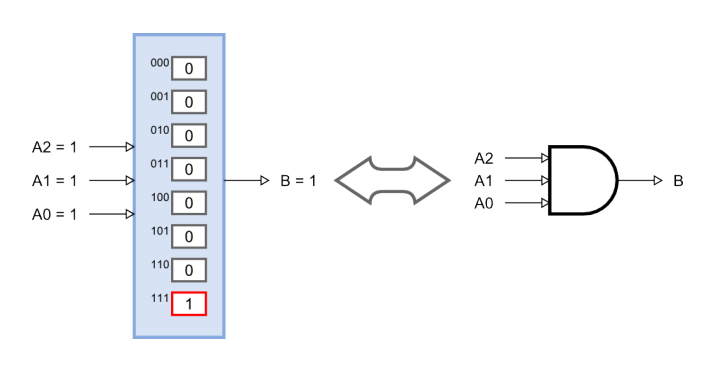
\includegraphics[width=1\textwidth, keepaspectratio]{imgs/clb-lut.png}
\caption{The look up table of a CLB.}
\label{fig:clb}
\end{figure}
\noindent
Modern FPGAs have more than just CLBs, IOBs and a switching matrix. There are more complex block types like multipliers and multiplexers. 

\subsubsection{Design flow}
\begin{enumerate}
\item \textbf{Program logic in hardware description language (HDL)} \\
A hardware description language doesn't behave like normal programming languages. It describes logic as a collection of Processes operating in parallel and contains language constructs for \textbf{synchronous logic}. Compiler tools (synthesis) can recognise certain code constructs and generates appropriate logic. Not all constructs can be implemented in FPGAs.
\item \textbf{Logic synth} \\
This step transforms the HDL into a \textbf{netlist}. A netlist is a description of circuit connections which has a list of logical units and how they are connected. 
\item \textbf{Implementation}
\begin{itemize}
\item A \textbf{translator} merges together multiple netlists.
\item A \textbf{mapper} combines the gates in the netlist so they will fit into the available lookup table structure
\item \textbf{Place and route} assigns the lookup table groups to real locations on the FPGA and assigns connections in the switching matrix. This step is very challenge and computationally expensive as there are often many different ways of fitting the tables. It is also sometimes hard to get it to fit at all.
\end{itemize}
\item \textbf{Bitstream generation} \\
Combines implementation output with configuration constraints to produce a bitstream which matched the desired FPGA.
\item \textbf{Downloader} \\
Transfers the bitstream to the FPGA and configures it for use.
\end{enumerate}

\subsubsection{Summary of FPGA}
FPGAs are large complex functions with re-programmabiliy and flexibility. 
\n
\textbf{Advantages}
\begin{itemize}
\item Massively parallel architecture
\item Processing many channels simultaneously with Fast Turnaround Designs
\item Uses standard IC Manufacturing processes to take advantage of Moore's Law
\item Mass produced and inexpensive.
\item Many variants with different sizes and features
\end{itemize}
\textbf{Disadvantages}
\begin{itemize}
\item Not radiation hard
\item Power hungry
\item No analogue signal processing
\end{itemize}
\section{Vector and Data Level Parallelism}
Single instruction, multiple issue (SIMD) architectures can exploit significant data-level parallelism for matrix-oriented computations of scientific computing and media-oriented image/sound processing. Additionally, SIMD is potentially more energy efficient than MIMD as it only needs to fetch one instruction per data operation, making it more attractive for mobile devices. Finally, SIMD allows the programmer to continue to think sequentially while achieving parallel speed-up. 
\n
There are three variations of SIMD:
\begin{itemize}
\item \textbf{Vector architectures} - These essentially mean to pipeline execution of many data operations. They were considered too expensive for microprocessors until recently, the expense coming from the transistors and cost of sufficient DRAM bandwidth. 
\item Multimedia \textbf{SIMD instruction set extensions} - This basically means simultaneous parallel data operations and is found in most ISAs today that support multimedia applications. 
\item \textbf{GPUs} - This offers higher potential performance than traditional multicore computers. 
\end{itemize}

\subsection{Vector architectures}
The basic idea behind vector architectures is to read sets of data elements into \textit{vector registers}, operate on those registers, then disperse the results back into memory. A single instruction operates on vectors of data, which results in dozen of register-register operations on independent data elements. 
\n
The vector registers act as compiler-controlled buffers to hide memory latency and leverage memory bandwidth. 

\subsubsection{VMIPS}
VMIPS is an instruction set architecture using MIPS for its scalar portions. Its vector portions are simply logical vector extensions to MIPS. 
\begin{itemize}
\item \textbf{Vector registers} - Each vector register is a fixed-length bank that holds a single vector. In VMIPS, each vector register can hold 64 elements, each 64 bits wide. The vector register file needs to provide enough ports to feed all the vector functional units. 
\item \textbf{Vector functional units} - Each unit if fully pipelined and can start a new operation every clock cycle. A control unit is needed to detect hazards on register accesses. 
\item \textbf{Vector load/store unit} - The vector memory unit loads or stores a vector to or from memory. Again, the VMIPS vector load and store is fully pipelined so that words can be moved between the registers and memory with a bandwidth of one word per clock cycle after an initial latency. 
\item \textbf{Set of scalar registers} - Scalar registers to provide data as input to the vector functional units. There are the normal 32 general-purpose registers and 32 floating point registers just like MIPS. 
\end{itemize}
\begin{figure}[H]
\centering
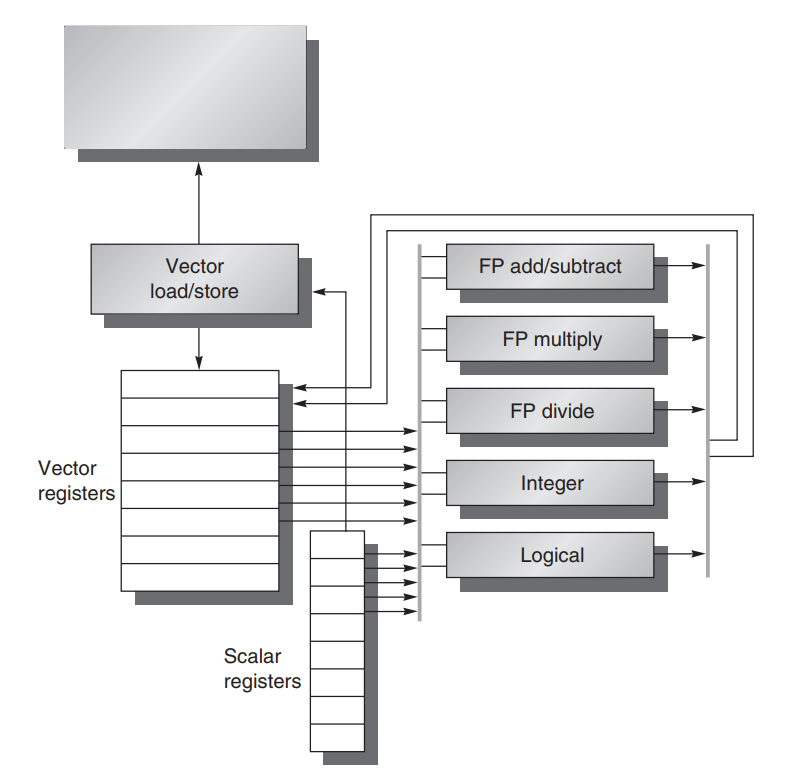
\includegraphics[width=0.8\textwidth, keepaspectratio]{imgs/vmips.png}
\caption{Basic structure of VMIPS.}
\end{figure}
\noindent
Instructions in VMIPS are similar to MIPS instructions, but with the letters ``VV" appended, for example \texttt{ADDVV.D}. The vector instructions either take a pair of vector registers, or a vector and scalar register (\texttt{ADDVS.D}) to operate on. Each vector instruction will only stall for the first element in each vector, then subsequent elements will flow smoothly down the pipeline. Loops can be vectorized when they do not have dependences between iterations of a loop, called \textbf{loop-carried dependences}.

\subsubsection{Vector execution time}
Execution time of vector operations primarily depends on three factors:
\begin{enumerate}
\item Length of operand vectors
\item Structural hazards in operations
\item Data dependences
\end{enumerate}
Given the vector length and initiation rate - the rate at which a vector unit consumes new operands and produces new results - we can compute the time for a single vector instruction. VMIPS implementation has one lane with a rate of one element per clock cycle for individual operations. Therefore, the execution time in clock cycles for a single vector instruction is approximately the vector length. 
\n
A notion of a \textbf{convoy} is used as a set of vector instructions that could potentially execute together. The instructions in a convoy \textit{must not} contain any structural hazards. If there are any hazards, the instructions need to be done sequentially and initiated in different convoys. However, RAW dependency hazards are allowed in the same convey via \textit{chaining}.

\subsubsection{Chaining}
Chaining allows a vector operation to start as soon as the individual elements of its vector source operand become available. The results from the first functional unit in the chain are ``forwarded" to the second functional unit. 
\n
A \textbf{chime} metric is used to estimate the time to execute on convoy. So $m$ convoys will execute in $m$ chimes. For a vector of length $n$, this will be $m \times n$ clock cycles. However, this chime approximation ignores some processor-specific over-heads, many of which are dependent on vector length. This means measuring time in chimes is better for long vectors than short ones. 

\subsubsection{Challenges}
Another source of overhead ignored by the chime model is vector \textit{start-up time}. The start-up time is principally determined by the latency of the vector functional unit. For example a floating-point add takes 6 clock cycles. 
\n
To improve on this, there are several optimisations that can improve performance or increase the types of programs that can run well on vector architectures:
\begin{itemize}
\item \textbf{Multiple lanes} to get more than one element per clock cycle
\item \textbf{Vector length register} to handle non-64 wide vectors
\item \textbf{Vector mask register} to handle conditionals (if statements) in vector loops
\item \textbf{Memory banks} to supply bandwidth to vector load/store units
\item \textbf{Striding} to handle multidimensional arrays
\item \textbf{Gather-Scatter} to handle sparse matrices
\item Programming vector architectures
\end{itemize}

\subsubsection{Multiple Lanes}
A key advantage of the vector instruction set is the ability to pass a large amount of parallel work to hardware using only a single short instruction. The parallel semantics allows a vector instruction to execute these elemental operations using a deeply pipelined functional unit. 
\n
The VMIPS instruction set has the property that element $N$ of one vector register can only take part in operations with element $N$ from other vector registers. This simplifies the construction of highly parallel vector units as multiple parallel \textit{lanes}. The peak throughput can therefore be increased by adding more lanes. 
\begin{figure}[H]
\centering
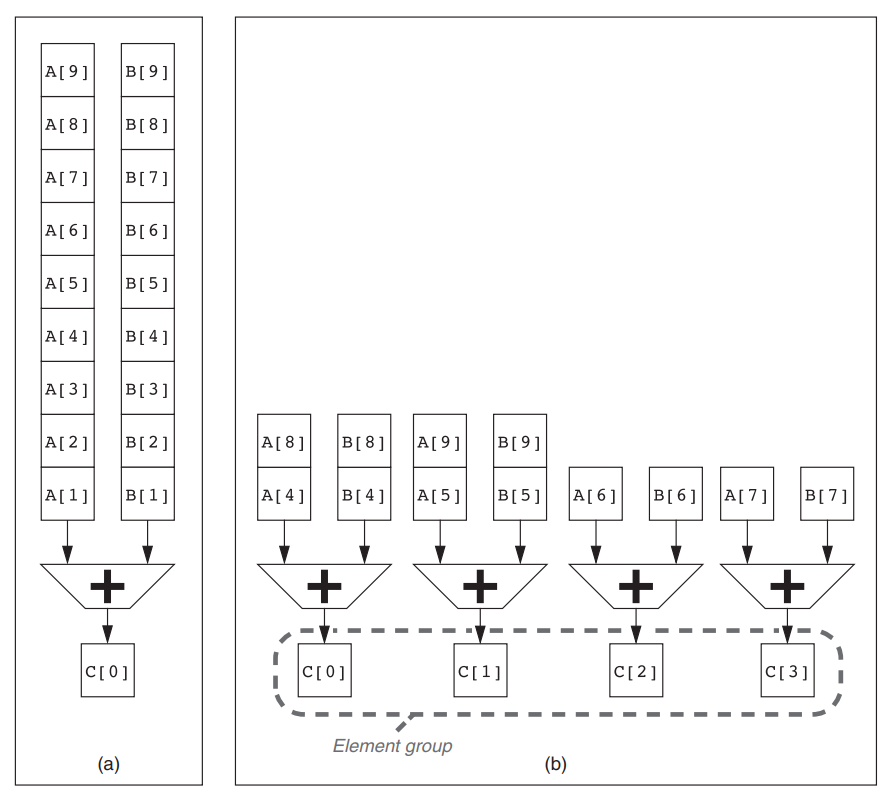
\includegraphics[width=0.9\textwidth, keepaspectratio]{imgs/vector-multiple-lanes.png}
\caption{Using multiple functional units to improve the performance of a single vector add instruction C = A + B}
\end{figure}
\noindent
For multiple lanes to be advantageous, both the applications and the architecture must support long vectors, otherwise, they execute too quickly and instruction bandwidth will run out, requiring ILP to supply enough vector instructions. 
\n
Adding multiple lanes is a good technique to improve vector performance as it requires little increase in control complexity and does not require changes to existing machine code. If the clock rate of a vector processor is halved, doubling the number of lanes will retain the same potential performance. 

\subsubsection{Vector-length registers}
What if the vector length is not known at compile time? 
\n
A vector processor has a natural vector length determined by the number of elements in each vector register. For example, this is 64 in VMIPS. This is unlikely to match the real vector length of a program.
\n
The solution is to create a \textbf{vector-length register} (VLR). The VLR controls the length of any vector operation, including load and store operations. The value in the VLR cannot be greater than the length of the vector registers, which is fine as long as the real length is less than or equal to the \textit{maximum vector length}. 
\n
To tackle the second problem of real lengths being longer than the maximum vector length, \textbf{strip mining} can be used. This creates two loops, one which can handle any number of iterations that is a multiple of the MVL ($n\ \text{mod}\ m$) and another than handles any remainder iterations less than the MVL. 

\subsubsection{Vector mask registers}
Programs that contain \texttt{if} statements in loops cannot be run in vector mode because they introduce control dependences. For example, consider the following loop:
\begin{lstlisting}
for (i = 0; i < 64; i++) {
	if (x[i] != 0) {
		x[i] = x[i] - y[i];
	}
}	
\end{lstlisting}
This loop cannot normally be vectorised because of the conditional. A common extension to allow this is \textbf{vector-mask control}. Mask registers provide conditional execution of each element operation in a vector instruction. The vector-mask control uses a boolean vector to control the execution of a vector instruction. When the mask is enabled, any vector instructions executed operate only on the vector elements whose corresponding entries in the vector-mask register are 1. Clearing the vector-mask register sets all values to 1, making subsequent vector instructions operate on all vector elements. 
\n
This does comes with an overhead, vector instructions executed with the mask still take up execution time, even for the elements where the mask value is 0. This causes the GFLOPS rate to decrease.

\subsubsection{Memory banks}
The behaviour of the vector load/store instructions are a lot more complicated than the vector arithmetic functional units. The start up time for a load is the time to get the first word from memory into a register. If the rest of the vector can be supplied without stalling, then the vector initiation rate will be the same as the rate at which new words are fetched or stored. 
\n
To maintain this hight initiation rate of one word fetched/stored per clock, the memory system must be able to produce or accept this much data. Having several numbers of banks is useful for dealing with vector loads or stores that access rows or columns of data. Most vector processes use memory banks, which allow multiple independent accesses for three reasons:
\begin{enumerate}
\item Ability to control the address to the banks separately
\item Be able to load or store data words that are not sequential.
\item Support multiple vector processors sharing the same memory system. 
\end{enumerate}

\subsubsection{Stride}
The position in memory of adjacent elements in a vector may not be sequential. For example:
\begin{lstlisting}
for (i = 0; i < 100; i++) {
	for (j = 0; j < 100; j++) {
		A[i][j] = 0.0;
		for (k = 0; k < 100; k++) {
			A[i][j]= = A[i][j] + B[i][k] * D[k][j];
		}
	}
}
\end{lstlisting}
To vectorise this multiplication, we must vectorise the rows of B with the columns of D. This distance is called a \textbf{stride} and represents the distance between elements to be gathered in a single register. Here, \texttt{D} would have a stride of 100 words and \texttt{B} would have a stride of 1 word. If it were column-wise the strides would be the opposite.  So here, without re-ordering the loops, the compiler can't hide the long distance between successive elements of \texttt{B} and \texttt{D}. 
\n
Once a vector is loaded into a vector register, it acts as it it had logically adjacent elements. This allows vector processors to handle strides greater than one (\textit{non-unit strides}). This ability to access nonsequential memory and reshape them into this dense structure is one of the major advantages of vector processors. 
\n
Supporting these non-unit strides complicates the memory system. It becomes possible to request access from the same bank frequently . When multiple access contend for a bank, a bank conflict occurs, stalling one of the accesses. A bank conflict will occur if:
\begin{equation*}
\frac{\text{Number of banks}}{\text{Least common multiple(Stride, number of banks)}} < \text{Bank busy time}
\end{equation*}

\subsubsection{Gather-Scatter}
It is important to have techniques to allow programs with sparse matrices to execute in vector mode. In a sparse matrix, the elements of a vector are stored in some compact form and accessed indirectly. 
\n
The mechanism for supporting sparse matrices is \textbf{gather-scatter operations} using index vectors. The goal is to support moving between a compressed representation (zeroes no included) and a normal representation (zeroes included) of a sparse matrix. 
\begin{itemize}
\item \textbf{Gather} - takes an \textit{index vector} and fetches the vector whose elements are at the addresses given by adding the base address to the offsets given in the index vector. The result is a dense vector in a vector register. 
\item After the elements are operated on in dense form, the sparse vector can be expanded by a \textbf{scatter} store with the same index vector. 
\end{itemize}
Essentially, \textit{gather} is an indexed load and \textit{scatter} is an indexed store. They run more slowly than the non-indexed versions since the memory banks are not known at the start of the instruction. 
\subsubsection{Programming vector architectures}
An advantage of vector architectures is that compilers can tell programmers at compile time whether a section of code will vectorise or not. By giving hints on how to improve performance, it simplifies programming of vector processors. 
\n
The main factor that affects the success of vector processes is the structure of programs themselves: Do the loops have true data dependences or can they be restructured to have no such dependences?

\subsection{SIMD extensions}
SIMD multimedia extensions came from the observation that many media applications operator on data types narrows than the native word size (e.g. 32 or 64 bits). For example, many graphics systems uses 8 bits for colour and 8 bits for transparency. Many audio samples are usually represented with 8 or 16 bits. Unlike vectors, SIMD instructions have smaller register files and specify fewer operands.
\n
Compared to vector instructions, SIMD extensions have three limitations:
\begin{itemize}
\item Fixed number of data operands in the opcode, unlike vector architectures which have variable length registers and have implicit maximum lengths
\item No sophisticated addressing mode like vector architectures (namely stride access and gather-scatter access)
\item No mask registers to support conditional execution
\end{itemize}
These limitations make it harder for the compiler to generate SIMD code and make it more difficulty to program in SIMD assembly languages. However, multimedia SIMD extensions are still very popular for the following advantages:
\begin{itemize}
\item Cost little to add to the standard ALU and easy to implement
\item Require little extra state with fast context switches
\item Less memory bandwidth requirements
\item Generally aligned memory access, so there is no chance of page faults in the middle of access
\item Short, fixed-length ``vectors" make it easy to introduce instructions to help with new media standards or to adapt to particular tasks
\end{itemize}
\subsubsection{Roofline performance model}
The roofline model is a visual way of comparing potential floating-point performance variations of SIMD architectures. The basic idea is to plot peak floating-point throughput as a function of arithmetic intensity. It ties together floating-point performance, memory performance and arithmetic intensity in a two-dimensional graph. \textbf{Arithmetic intensity} is the ratio of floating-point operations per byte of memory accessed.
\begin{figure}[H]
\centering
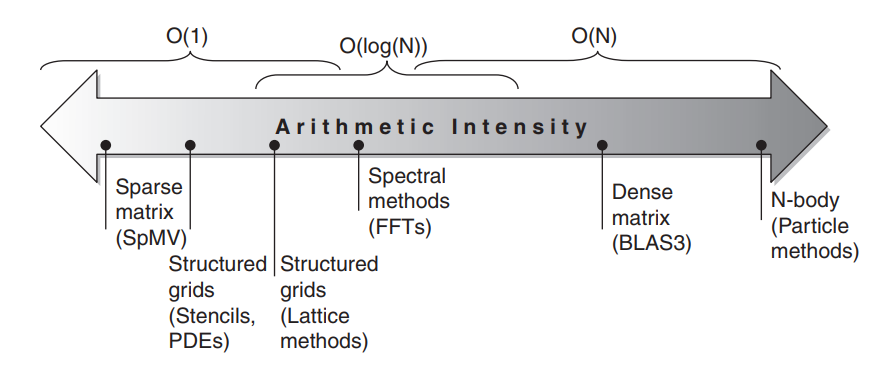
\includegraphics[width=1\textwidth, keepaspectratio]{imgs/roofline-model.png}
\caption{Arithmetic intensity, specified as the number of floating-point operations to run the program divided by the number of bytes accessed in main memory}
\end{figure}
\noindent


\begin{figure}[H]
\centering
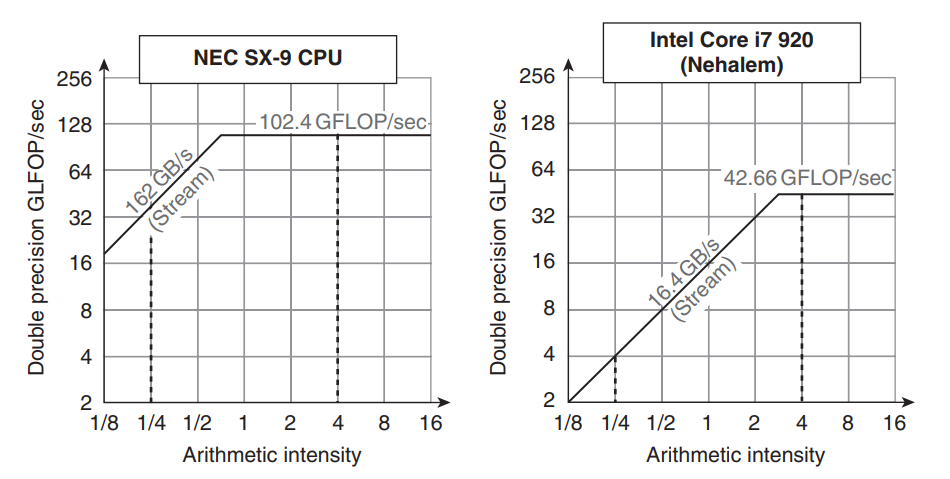
\includegraphics[width=0.9\textwidth, keepaspectratio]{imgs/roofline-model2.png}
\caption{Roofline model for two different processors}
\end{figure}
\noindent
We can think of arithmetic intensity as a pole that hits the roof. If it hits the flat part, then performance is computationally limited. If it hits the slanted part of the root, then performance is limited by memory bandwidth. The further left the ``ridge-point" is, the more kernels can potentially hit the maximum performance. 

\subsection{GPUs}
To be able to program for GPUs, programmers have to worry about both getting good performance and scheduling between the CPU and GPU. NVIDIA developed a C-like language called CUDA that unifies all forms of parallelism as a CUDA thread. This kind of programming model is called Single Instruction, Multiple Thread (SIMT). These threads are blocked together and executed in groups of 32 threads, called a \textit{thread block}. The hardware the executes a whole block of threads is a \textbf{multithreaded SIMD processor}. 
\n
Each CUDA thread is associated with each data element. The threads are organised into blocks which are organised into a grid. 
\begin{figure}[H]
\centering
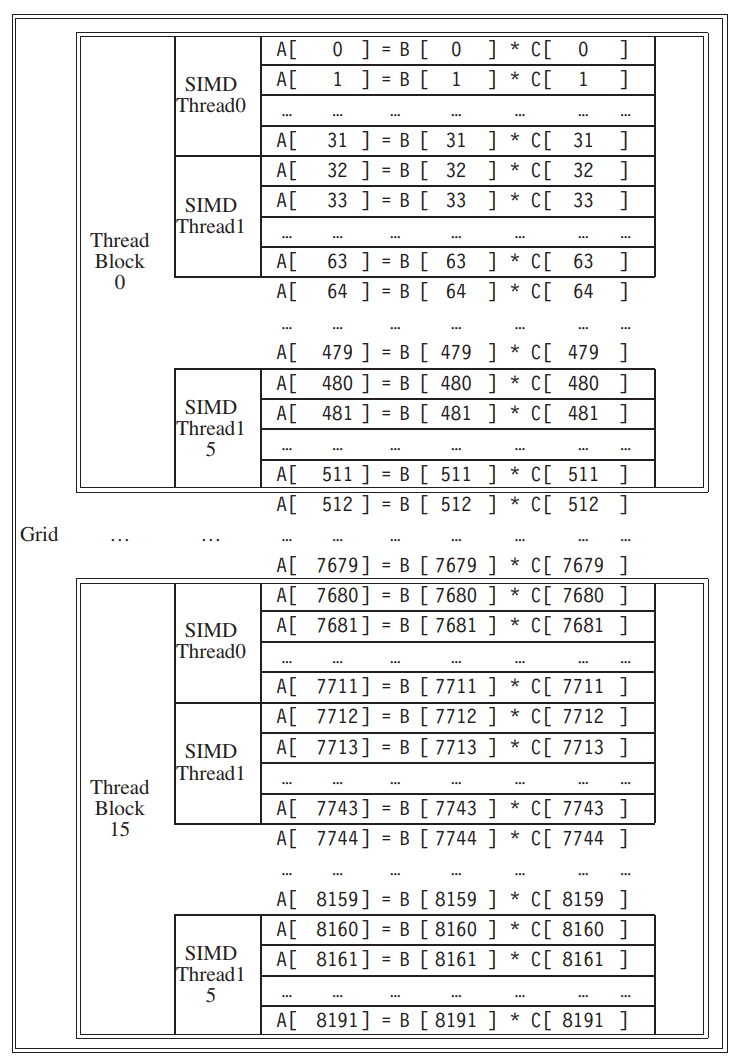
\includegraphics[width=0.8\textwidth, keepaspectratio]{imgs/cuda-grid.png}
\caption{Mapping of a grid, thread blocks and threads of SIMD instructions.}
\end{figure}
\noindent
A \textbf{Grid} is the code that runs on a GPU that consists of a set of \textbf{Thread blocks}. The grid and thread block are programming abstractions implemented in GPU hardware to help programmers organise CUDA code. A thread block is assigned to a multithreaded SIMD processor by the \textbf{Thread Block Scheduler}.This is similar to a control processor in a vector architecture. It determines the number of thread blocks needed for the loop and allocates them to different multithreaded SIMD processors until the loop in complete. 

\subsubsection{NVIDIA GPU Memory structures}
Each SIMD lane has a private section of off-chip DRAM which is its private memory. This memory contains things such as the stack frame, spilling registers and private variables. 
\n
Each multi-threaded SIMD processor also has its own local memory which is shared by a SIMD lanes/threads within the block. 
\n
Memory shared by all the SIMD processors is the \textbf{GPU memory}. The host (CPU) can read and write to GPU memory. 

\begin{figure}[H]
\centering
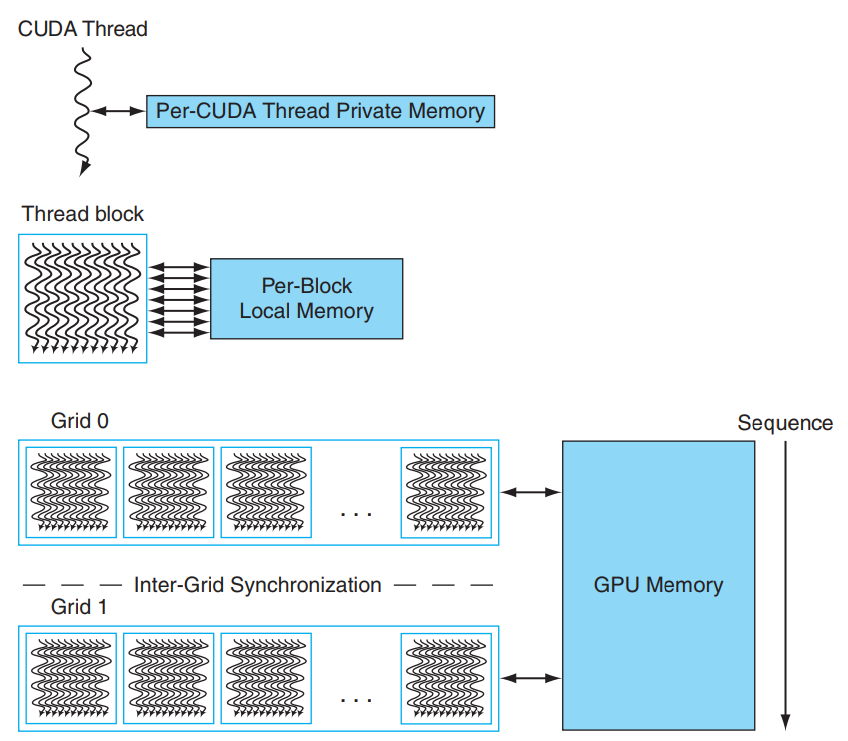
\includegraphics[width=0.9\textwidth, keepaspectratio]{imgs/gpu-memory.png}
\caption={GPU Memory structures.}
\end{figure}
\noindent
Rather than use large caches to contain whole working sets of an application, GPUs use a smaller cache and rely on extensive multi-threading of threads of SIMD instructions to hide the long latency to DRAM. 
\subsubsection{Similarities and differences between Vector architectures and GPUs}
\textbf{Similarities}:
\begin{itemize}
\item Works well with data-level parallel problems
\item Gather-scatter transfers
\item Mask registers
\item Large register files
\end{itemize}
\textbf{Differences}:
\begin{itemize}
\item No scalar processor - must disable all but one SIMD lane on a processor 
\item Uses multi-threading to hide memory latency. Vector processes have no multi-threading. 
\item Has many functional units - compared to few deeply pipelined units in vector processors. 
\end{itemize}

\subsubsection{Optimisations in the Fermi GPU architecture}
The multi-threaded SIMD processor of Fermi is more complicated. To \textit{increase hardware utilisation}, each SIMD processor for two SIMD thread schedulers and two instruction dispatch units. The two schedulers selects two threads of instructions and issues one instruction from each to two sets of 16 SIMD lanes. This way, two threads of SIMD instructions are scheduled every two clock cycles. This innovation is analogous to a multi-threaded vector processor that can issue vector instructions from two independent threads. 
\n
Fermi introduces several innovations to bring GPUs closer to mainstream system processors:
\begin{itemize}
\item \textbf{Fast double precision floating-point arithmetic}
\item \textbf{Caches for GPU memory} - Fermi includes both L1 Data cache and L1 instruction cache for each multi-threaded SIMD processor and L2 shared cache for all SIMD processors in the GPU. This reduces bandwidth pressure from the GPU DRAM and also saves energy by not having to going to off-chip memory. 
\item \textbf{64-bit addressing and a unified address space}
\item \textbf{Error correcting codes} to detect and correct errors in memory and registers.
\item \textbf{Faster context switching} - Hardware support to switch contexts faster
\item \textbf{Faster atomic instructions} - Improved performance of atomic instructions with a special hardware unit associated with the L2 cache. 
\end{itemize}

\subsection{Detecting and enhancing loop level parallelism}
Finding and manipulating loop level parallelism is critical to exploiting both DLP and TLP as well as aggressive static ILP approach likes VLIW. Loop-level parallelism is normally analysed at the source level while most analysis of ILP is done after instructions have been generated by the compiler. Loop-level analysis involves determining what \textbf{dependences} exist among the operands in a loop across the iteration. 
\n
The analysis of loop-level parallelism therefore focuses on determining whether data accesses in later iterations are dependent on data values produced in earlier iterations. This is called a \textbf{loop-carried dependence}. For example: \\
\begin{lstlisting}[caption={Example of a parallel loop}, captionpos=b]
for (i = 999; i >= 0; i--) {
	x[i] = x[i] + s
}
\end{lstlisting}
\noindent
In this loop, the two uses of \texttt{x[i]} are dependent, but this dependence only exists within a single iteration and is not loop carried.
\\
\begin{lstlisting}[caption={Example of a loop with loop-carried dependences}, captionpos=b]
for (i = 0; i < 100; i++) {
	A[i + 1] = A[i] + C[i]; 	// S1
	B[i + 1] = B[i] + A[i + 1]; // S2
}
\end{lstlisting}
\noindent
There are two different dependences in this example:
\begin{enumerate}
\item \texttt{S1} and \texttt{S2} use values computed in a previous iteration. Iteration \texttt{i} computes \texttt{A[i + 1]} which is used in iteration \texttt{i + 1}.
\item \texttt{S2} uses the value \texttt{A[i + 1]} which is computed by \texttt{S1} in the same iteration.  
\end{enumerate}
Because the second dependence is within the same iteration and not loop carried, it can still be parallelised with as long as each pair of statements in an iteration were kept in order. The first dependence is loop carried and therefore this loop cannot be parallelised. 
\n
However, it is possible to have loop-carried dependences that do not prevent parallelism:
\begin{lstlisting}
for (int i = 0; i < 100; i ++) {
	A[i] = A[i] + B[i];		// S1
	B[i + 1] = C[i] + D[i] 	// S2
}
\end{lstlisting}
\texttt{S1} uses a value assigned in the previous iteration by \texttt{S2} so there is a loop-carried dependence between \texttt{S2} and \texttt{S1}. Despite this, the loop can still be made parallel. This is because the dependence is not circular - the statements do not depend on themselves or each other. To parallelise the loop, it must be transformed to conform to the partial ordering:
\begin{lstlisting}
A[0] = A[0] + B[0];
for (int i = 0; i < 99; i++) {
	B[i + 1] = C[i] + D[i];
	A[i + 1] = A[i + 1] + B[i + 1];
}
B[100] = C[99] + D[99];
\end{lstlisting}
Now the dependence is no longer loop-carried, so the iterations of the loop can be overlapped. 

\subsection{GPU Programming}
How a programmer programs on a GPU says a lot about how it works. \texttt{OpenCL} is a C-like language like \texttt{CUDA}, but it targets \textbf{heterogeneous} hardware. The idea is that it can be written once and run on any processor. 
\n
- opencl calls like black box
- write kernel separately
- not properly supported by any platform
\n
The specification is split into four main parts:
\begin{itemize}
\item Platform model
\item Execution model
\item Memory model
\item Programming model
\end{itemize}

\subsubsection*{Platform model}
Specifies the host/device relationship. A \textbf{host} is the processor the coordinates the execution while the \textbf{device} is the processor which executes the OpenCL code. There can be multiple devices where the OpenCL code is run on. 
\n
The platform model defines an abstract hardware model.
\begin{itemize}
\item OpenCL functions are called \textbf{kernels}
\item \textbf{Kernels} execute on \textbf{devices}
\end{itemize}
Only the devices need to be OpenCL compatible. 
\n
A \textbf{device} is divided into one or more \textbf{computer units}. Computer units are then further divided into one or more \textbf{processing element}. Each processing element maintains its own program counter. 
\begin{figure}[H]
\centering
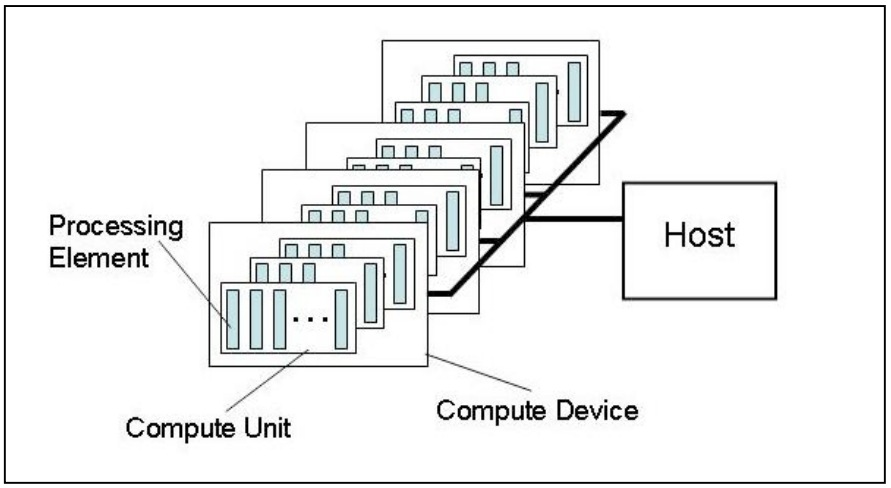
\includegraphics[width=0.8\textwidth, keepaspectratio]{imgs/opencl-platform-model.jpg}
\caption{OpenCL platform model}
\end{figure}

\subsubsection*{Execution model}
The execution model defines how OpenCL is configured on the host and how kernels are executed. Since OpenCL applications run on a host which submits work to the compute devices.
\begin{itemize}
\item \textbf{Context} - The environment within which work-items execute. This includes devices and their memory/command queues
\item \textbf{Program} - collection of kernels and other functions (analogous to a dynamic library)
\item \textbf{Kernel} - The code for a work item, basically a C function
\item \textbf{Work item} - The basic unit of work on an OpenCL device
\end{itemize}
The applications queue kernel execution, which can be in-order or out-of-order. 

\subsubsection*{Concurrency model}
OpenCL has a hierarchical concurrency model consisting of:
\begin{itemize}
\item Work groups
\item Work items
\end{itemize}
This hierarchical model promotes scalability. Each kernel is specified an \textit{n-dimensional range} (NDRange). It is a n-dimensional index of work items which generally corresponds to the dimensionality of the input/output space. 
\n
For example, to add arrays of 1024 elements:
\begin{enumerate}
\item First, divide the work-items into equal work groups. The work groups must have the same dimensionality as NDRange, so for example for a single array of elements, the dimensionality can simply be 1. Here we can choose a work group size of 64 (64 work items in the work group). 
\item Since there are 1024 work items per vector and the work group size is 64, therefore there are 16 work groups.
\begin{equation*}
\frac{1024}{64} = 16
\end{equation*}
\begin{figure}[H]
\centering
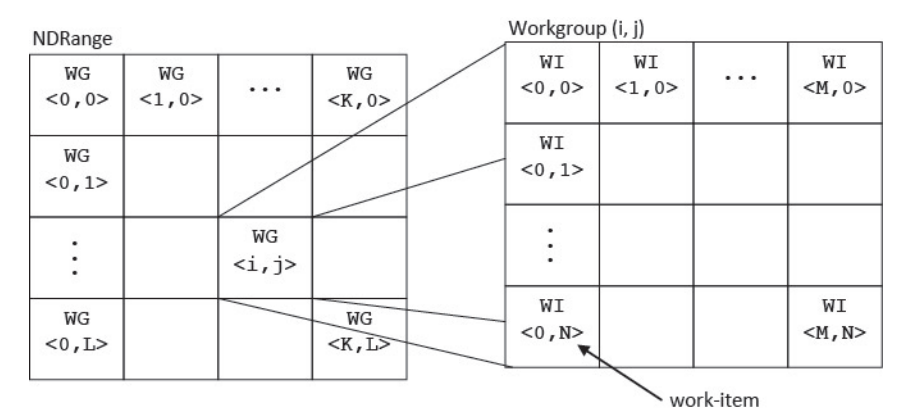
\includegraphics[width=1\textwidth, keepaspectratio]{imgs/work-groups.png}
\caption{Workgroups.}

\end{figure}
\end{enumerate}
The hardware usually defines the most efficient workgroup size. The index space size for workgroups should be evenly divisible by the work group size. Otherwise, some work items in the workgroup will be doing no work. This model is scalable as work groups are independent from one another while all work items in the same work-group can communicate to each other. The index space defines a hierarchy of work-groups and work-items.  
\begin{figure}[H]
\centering
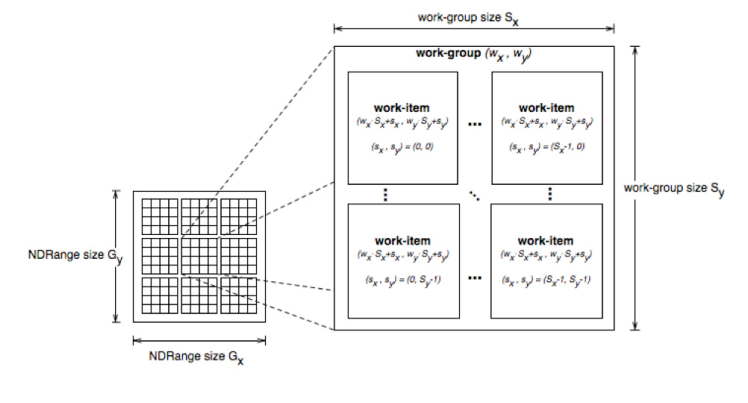
\includegraphics[width=0.8\textwidth, keepaspectratio]{imgs/work-items.png}
\caption{Work items.}
\end{figure}
\noindent
Work items with the same work group have a \textit{shared memory space} that allows for fast communication. They can also perform \textbf{barrier synchronisation}  Each work item can uniquely identify themselves based on:
\begin{itemize}
\item A global id (unique within the whole index space)
\item A work group id 
\item A local id within the same work group
\end{itemize}
Massively parallel programs are usually written so that each thread computer one part of the problem. For example for vector addition of two arrays, each thread will perform one addition of corresponding elements from the two arrays. 

\subsubsection*{Memory model}
The memory model abstracts the memory hierarchy to be \textbf{independent} from the underlying memory architecture. In reality, the model closely resembles modern GPU architecture. 
\begin{itemize}
\item \textbf{Private memory} - Private memory per work-item
\item \textbf{Local memory} - Memory shared within a work group
\item \textbf{Global/constant memory} - Global memory visible to all work groups.
\item \textbf{Host memory} - Main memory on the host processor.
\end{itemize}
\begin{figure}[H]
\centering
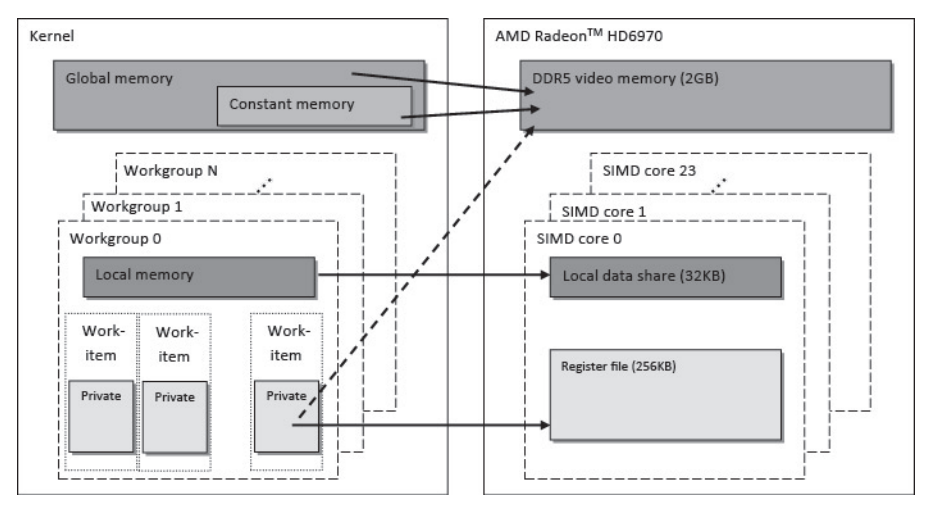
\includegraphics[width=1\textwidth, keepaspectratio]{imgs/opencl-memory-model.png}
\caption{OpenCL memory model vs reality.}
\end{figure}
\noindent
Memory management must be done explicitly. The programmer allocates memory to different spaces in the abstract memory hierarchy. For example moving data from host \rightarrow global \rightarrow local. The runtime system will map these spaces into the physical memory hierarchy. 

\subsubsection*{Programming model}
The programming model is how the concurrency model is mapped to the physical hardware. The \textbf{contexts} which execute the kernel are mapped to actual device hardware units. 
\n
For example, a typical setup would be to have an x86 CPU as the host and a GPU OpenCL processor as the device. The host sets up the kernel for the device to run and instantiates the kernel with some specified degree of parallelism. The GPU device then executes the kernel when instructed to by the host. All IO is done via the host. 



\section{Exploiting GPUs}

\section{Multicore programming}
There are many forms of low level parallelism that could be done:
\begin{itemize}
\item pThreads
\item OpenMP
\item MPI
\item OpenCL
\item Assembly/vector instructions
\end{itemize}
There is a difference between \textbf{task parallelism} and \textbf{Data parallelism}. Task parallelism is about the distribution of \textit{independent} processes across different processing units and this includes forms such as \textbf{pThreads}, \textbf{MPI} and \textbf{OpenCL}. Data parallelism is about the distribution of different data across multiple processing units where the same or similar operations are performed using forms such as \textbf{OpenMP}, \textbf{MPI} and \textbf{OpenCL}.

\subsection{pThreads}
pThreads are POSIX threads and allows multiple threads to exist in a program at a very low level. The threads can be independent or collaborative where collaboration is more difficult as it requires communication between the threads.
\n
pThreads are asynchronous and non-deterministically scheduled. This means that the run time is in charge of scheduling and each run will produce different result in terms of which threads get to run. Scheduling these threads is a huge optimisation problem. 

\subsection{OpenMP}
OpenMP uses \textbf{shared memory} and \textbf{loop based} parallelism. The threads used in OpenMP are on a higher level than pThreads. The basic idea is to run a loop in parallel if it has no dependences. This follows the fork/join thread model:
\begin{figure}[H]
\centering
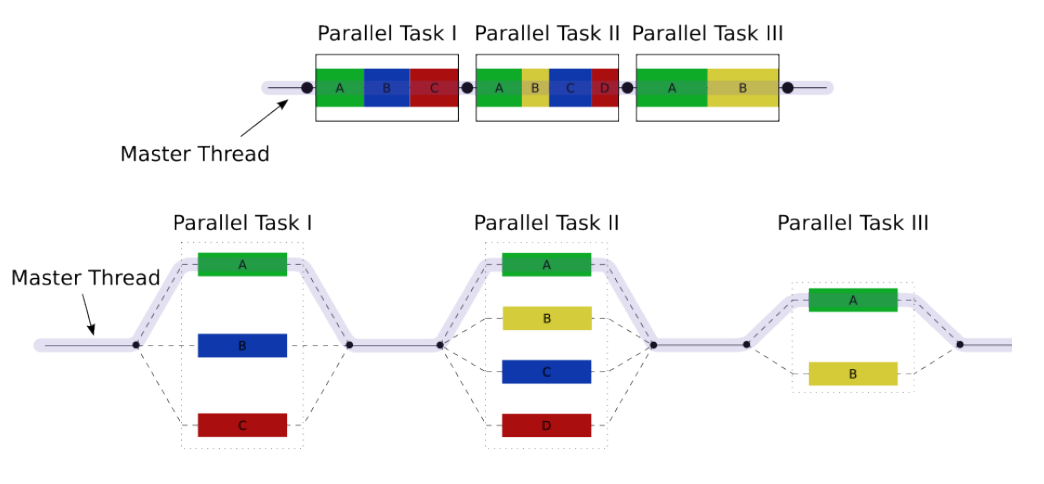
\includegraphics[width=1\textwidth, keepaspectratio]{imgs/fork-join-model.png}
\caption{OpenMP fork join model}
\end{figure}
\noindent
All OpenMP programs begin as a single process: the \textbf{master thread}. The master thread executes sequentially until the first parallel region construct is encountered. The master thread then \textbf{forks} to create parallel threads. The program then executes in parallel and when all threads finish, they are \textbf{joined} and terminate, leaving only the master thread.

\subsection{MPI}
MPI is the Message Passing Interface and does communication and synchronisation via message passing. This is generally for distributed memory, though it can be used with shared memory, though this would incur high overhead. 
\n
MPI is heavily used in High Performance Computing and network communication. 

\subsection{OpenCL}
OpenCL targets heterogeneous processors with a host/accelerator model. 

\subsection{Hybrids}
Use different forms for different problems. For example, since MPI is not efficient for shared memory and OpenMP cannot deal with distributed memory, use MPI for the network while using OpenMP for the shared memory on the system. However, this adds additional complexity. 

\subsection{PGAS}
PGAS stands for Partitioned Global Address Space and is an abstract for distributed memory. With PGAS, all memory is presented to the programmer as shared. PGAS handles the translation to distributed memory so it is much simpler for the programmer.
\n
Memory spaces are given \textbf{affinity}. Faster affinity means faster communication for that memory space.

\subsection{Hyperthreading}
For normal processors, when different program threads share the core one thread halts, the other can be switched in with a context switch. \textbf{Simultaneous multi-threading} (SMT) is a technique to increase performance by filling up processing time lost to memory latency. 
\n
One physical processor is presented to the system as two logical processors. If one thread stalls, the processor can switching to running the other.

\subsection{GPUs vs CPUS}
\textbf{GPUs}
\begin{itemize}
\item Hundreds of cores
\item Very simple cores
\item High memory bandwidth
\end{itemize}
\textbf{CPUs}
\begin{itemize}
\item Around 2-8 cores
\item Highly complex cores (superscalar, speculative, branch prediction, multiple issue)
\item Good memory bandwidth
\end{itemize}

\subsubsection{GPU cores}
A GPU core is designed to be kept busy by swapping in hundreds of threads while waiting for memory. This is how its high memory bandwidth hides the memory latency. This means the kind of programs that a GPU is able to run efficiently is different from that of CPUs. 

\subsection{Multi-objective optimisation}
To consider both execution time and power, we need multi-objective optimisation. 
\n
We can build a linear combination of optimisation goals as a na\"{i}ve approach. However, a better way it to generate a \textbf{Pareto front} and make a decision based on that front. 
\begin{figure}[H]
\centering
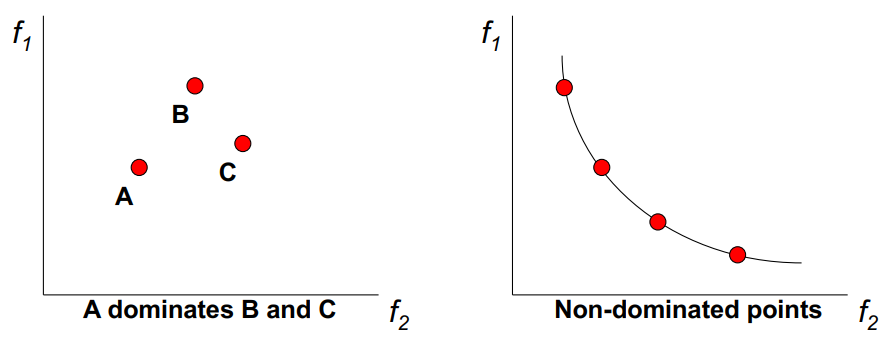
\includegraphics[width=0.9\textwidth, keepaspectratio]{imgs/pareto-front.png}
\caption{Pareto fronts}
\end{figure}
\noindent
For problems where more than one objective function are in conflict with each other, we can use a pareto based approach. This process does not seek a single solution, but gets a set of non dominated solutions and the front can be chosen based on trade-offs between the two objectives.
\section{Approximate Computing}
Usually in architecture, we try to optimise for execution time and power. There is also a third goal - \textbf{accuracy}. There are many soft applications where 100\% correction of computation is not necessary. These are applications such as image compression/processing, machine learning, multimedia and computer vision. 
\n
\textbf{Approximate computing} leverages the presence of error-tolerant code regions in applications to intelligently trade off implementation, storage, and/or result accuracy for performance or energy gains. In other words, be exploiting the gap between the level of accuracy required by the user and that provided by the computer system, accuracy can be reduced to gain increased performance of energy efficiency. 
\n
It is key to remember that even on suitable applications, only some sections of the code might be appropriate for approximate computing. Additionally, control flow and memory calculations are almost never suitable. Sometimes incorrect data can lead to never terminating programs.

\subsection{RAM optimisation}
\subsubsection*{DRAM}
We know that refreshing DRAM uses energy. By reducing the refresh rate, the energy used can be decreased. Of course this comes at a cost of a word being wrong or out of date more often.

\subsubsection*{SRAM}
Similarly, we know that SRAM requires a steady voltage and it can be decreased to lower energy. However, there are challenge to achieving low-voltage operation in SRAM due to process variation and bit cell stability. 

\subsection{Other easy optimisations}
\begin{itemize}
\item \textbf{Speculation} - Don't roll back despite wrong prediction and continue with wrong values anyway. 
\item \textbf{Cache} - Don't bother updating cache result even if there is a change.
\item \textbf{Prcision scaling} - Dynamically vary the precision of floating point numbers or find the minimum precision required at design time
\item \textbf{Loop perforation} - Skip some iterations of loops. This works for applications like Monte Carlo simulation and iterative refinement
\item \textbf{Load value approximation} - On a cache miss, predict the content of the memory location so reduce stalling
\item \textbf{Memorisation} - Store the output values of functions and assume later calls of the function have the same inputs and therefore the same outputs. 
\end{itemize}

\subsection{Identifying approximable codes}
Identifying can be programmer-led using C pragmas like OpenMP, or we can try to find them automatically.
\n
There is a software framework to try and find approximable codes automatically
\begin{itemize}
\item Collect the variables of a program and record normal ranges
\item Change the values of the variables using binary manipulation
\item Analyse the output and compare the closeness to known good output
\end{itemize}
This approach is like binary \textbf{mutation} testing to see how much the variables can be changed by without having bad output. 

\section{Multiprocessors}
Due to diminishing returns in exploiting ILP combined with growing concerns over power, new architectures have started to focus on exploiting thread-level parallelism (TLP) by having multiple CPU cores.
\n
TLP implies the existence of \textbf{multiple program counters} and therefore is exploited primarily with \textbf{MIMD} (Multiple instruction, multiple data). \textit{Multiprocessors} are defined as computers consisting of tightly coupled processors whose coordination and usage are controlled by a single OS and share memory though a shared address space. These systems exploit thread-level parallelism through two different software models:
\begin{itemize}
\item \textbf{Parallel processing} - execution of a tightly coupled set of threads collaborating on a single task
\item \textbf{Request-level parallelism} - execution of multiple, relatively independent processes from one or more users
\end{itemize}
To take advantage of a MIMD multiprocessor with $n$ processors, there must be at least $n$ threads or processes to execute. The amount of computation assigned to a thread is called a \textbf{grain size}. It is important in considering how to exploit TLP efficiently. Threads can be used to exploit DLP, although the overhead is likely to be higher than using some SIMD processor. This overhead means that the grain size must be sufficiently large to exploit the parallelism efficiently. 
\n
There are two classes of multiprocessors:
\begin{itemize}
\item \textbf{Symmetric (shared-memory) multiprocessors (SMPs)} - Features a small number of cores (8 or fewer). This makes it possible for the processors to share a single centralised memory that all processors have access to. All processors also have uniform latency from memory. 
\begin{figure}[H]
\centering
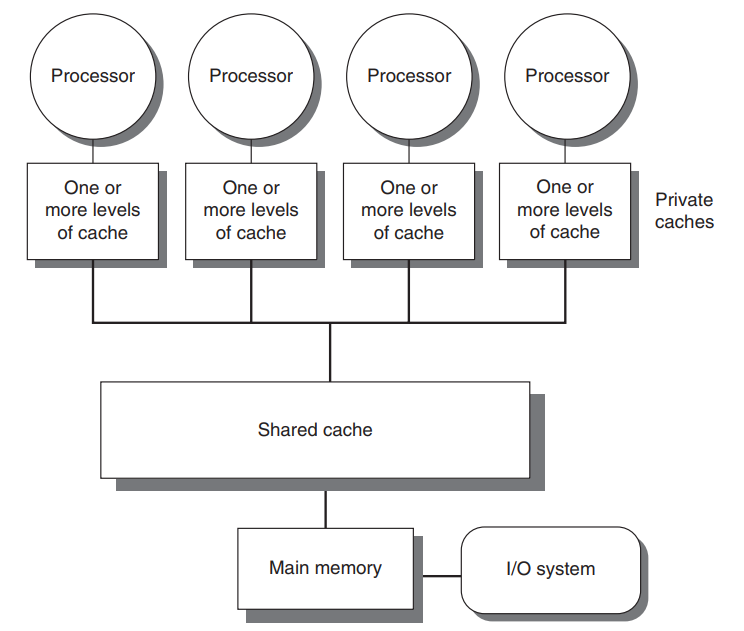
\includegraphics[width=0.9\textwidth, keepaspectratio]{imgs/smp.png}
\caption{Basic structure of a centralised shared memory multiprocessor.}
\end{figure}
\item \textbf{Distributed shared memory (DSM)} - Larger processor counts, which leads to memory being distributed among processors. Otherwise the memory system would not be able to support the bandwidth demands of so many processors without long latency. Distributing the memory increases the bandwidth and reduces the latency to local memory. However, the access time depends on the location of the data word (\textbf{NUMA} - Non-uniform memory access). The key disadvantage is the need to communicate data among processors and requires more effort in the software.  
\begin{figure}[H]
\centering
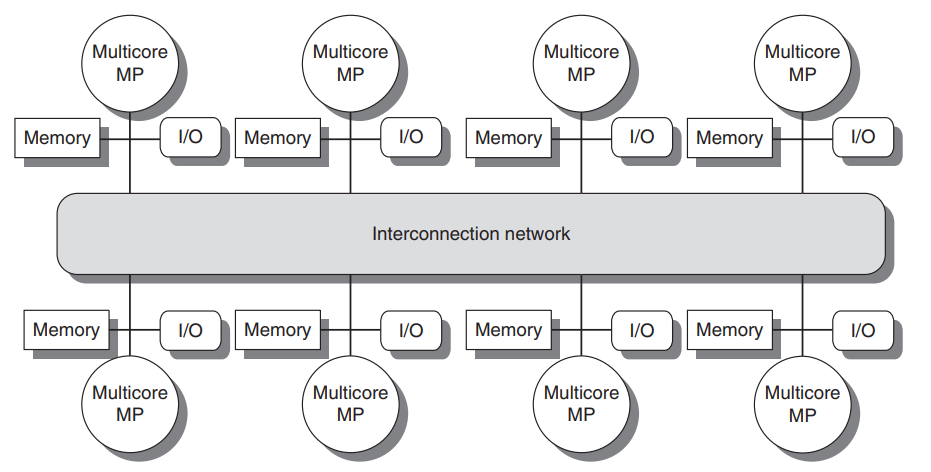
\includegraphics[width=1\textwidth, keepaspectratio]{imgs/dsm.png}
\caption{Basic architecture of a distributed memory multiprocessor.}
\end{figure}
\end{itemize}
In both architectures, communication between threads happens through a shared address space, so memory references can be made from any processor to any memory location. 

\subsection{Cache coherence}
Caching shared data in SMPs adds a new problem because memory held by two different processors is through their individual caches, which could end up seeing two different values. 
\begin{figure}[H]
\centering
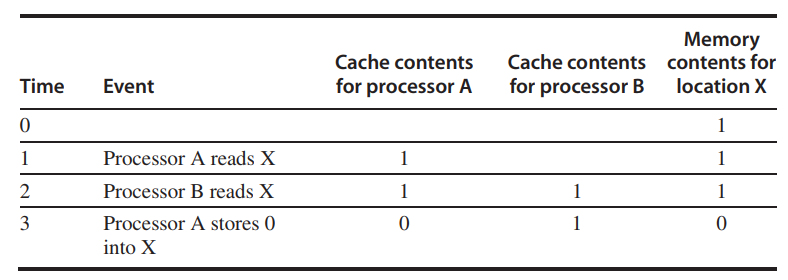
\includegraphics[width=1\textwidth, keepaspectratio]{imgs/cache-coherence.png}
\caption{Cache coherence problem for a single memory location}
\end{figure}
\noindent 
There are two aspects of cache coherency. \textbf{Coherence} and \textbf{Consistency}.
\begin{itemize}
\item \textbf{Coherence}
	\begin{itemize}
	\item All reads by any processor must return the most recently written value.
	\item Writes to the same location by any two processors are seen in the same order by all processors
	\end{itemize}
\item \textbf{Consistency}
\begin{itemize}
\item When a written value will be returned by a read
\item If a processor writes location A followed by location B, any processor that sees the new value of B must also see the new value of A. 
\end{itemize} 
\end{itemize}
Coherence defines the behaviour of reads and writes to the same memory location, while consistency defines the behaviour of reads and writes with respect to accesses to other memory locations. 

\subsubsection{Enforcing cache coherence}
A program running on multiple processors will normally have copies of the same data in several caches. In a coherent multiprocessor, the caches provide both \textbf{migration} and \textbf{replication} of shared data items. Migration refers to the movement of data, reducing the latency to access a shared data item. Replication refers to having multiple copies of the same data and reduces both latency of access and contention for a read shared data item. 
\n
There are two classes of \textit{cache coherence protocols}:
\begin{itemize}
\item \textbf{Directory based} - Sharing status of each block kept in one location
\item \textbf{Snooping} - Each core tracks the sharing status of each block
\end{itemize}

\subsubsection{Snoopy coherence protocols}
One method of snoopy protocols is to ensure that a processor has exclusive access to a data item before it writes to that item. This is called a \textbf{write invalidate protocol} as it invalidates other copies on a write. Exclusive access ensures that no other readable or writable copies of the data exists when the write occurs: all other cached copies are invalidated. 
\n
If two processors attempt to write the same data simultaneously, one of them wins the race, causing the other's copy to be invalidated. For the other processor to complete its write, it must now obtain a new copy of the data, which would contain the updated value. 
\n
An alternative to the invalidate protocol is to update all cached copies of a data item when that item is written. This is called a \textbf{write update} or \textbf{write broadcast} protocol. A write update protocol must broadcast all writes to shared cache lines and consumes more bandwidth. This is why most multiprocessors prefer write invalidate or write update. The absence of a centralised data structure to track the state of the caches is the fundamental advantage and disadvantage of a snooping-based scheme, since it allows it to be inexpensive, but the bus becomes a large bottleneck for scalability. 
\subsubsection*{Implementation of write invalidate}
The key to implementing an invalidate protocol in a multicore architecture is the use of the bus or some other broadcast medium to perform invalidates. To perform an invalidate, the processor must acquire bus access and broadcast the address to be invalidated on the bus. All processors continuously snoop on the bus, watching for addresses and invalidates them if a broadcast address is found in their cache. 
\n
When a write to a block that is shared occurs, the writer must acquire bus access to broadcast its invalidation. If two processors try to write at the same time, their broadcasts will be serialised, so one processor will obtain bus access first, causing any other copies to be invalidated. 
\n
Apart from invalidating items of a cache block being written to, we also need to locate a data item when a cache miss occurs. In \textit{write-through} cache, this is easy as all written data always goes back to memory, so the most recent value can be fetch. For \textit{write-back} cache, this is harder. Processors need to retrieve the data value from another processor's private (L1 or L2) cache. 
\n
Cache lines can be marked as \textbf{shared} or \textbf{exclusive}. When a write to a shared block occurs, the cache generations an invalidation and marks the bus as \textit{exclusive}. 
\begin{figure}[H]
\centering
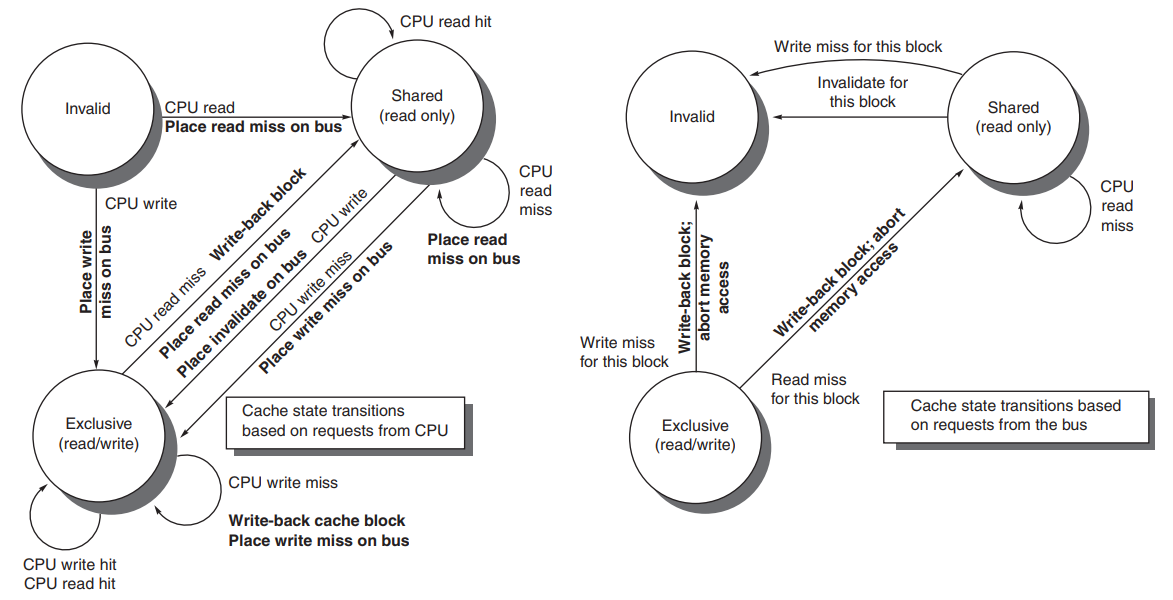
\includegraphics[width=1\textwidth, keepaspectratio]{imgs/snoopy.png}
\caption{A write invalidate, snoopy cache coherence protocol for write-back cache.}
\end{figure}

\subsubsection{Directory based coherence protocol}
A directory keeps the state of every block that may be cache. Information in the directory include which caches have copies of the block, whether it is dirty or not and so on. The simplest implementation is to have a directory at the outermost L3 cache: Simply keep a bit vector with size equal to the number of cores for each L3 data block and invalidation are only sent to those caches. 
\n
However, having a single directory on L3 cache is not scalable. The directory should be distributed in a way that the coherence protocol knows where to find the directory information for any cached block of memory. 
\begin{figure}[H]
\centering
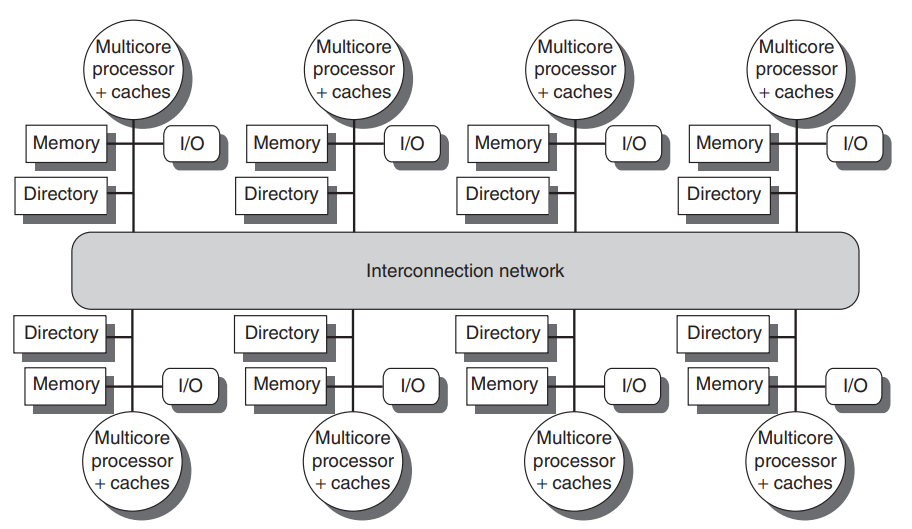
\includegraphics[width=1\textwidth, keepaspectratio]{imgs/directory-based.png}
\caption{A directory based cache coherence protocol where a directory is added to each node in a distributed-memory multiprocessor.}
\end{figure}
\noindent
Just like a snooping protocol, there are two primary operations that need to be handled: A read miss and handling a write to a shared, clean cache block. To implement this, a state for each block is maintained as follows:
\begin{itemize}
\item \textbf{Shared} - One or more nodes have the block cached and the value in memory is up to date
\item \textbf{Uncached} - No node has a copy of this cache block
\item \textbf{Modified (Exclusive)} - Exactly one node has a copy of the cache block and it has been written to, so the copy in memory is out of date. 
\end{itemize}
To keep track of which nodes have copies of a block, a bit vector can be used for each memory block. When the block is shared, each bit of the vector represents whether the corresponding processor has a copy of the block. The bit vector can also be used to keep track of the owner of a block when it is in exclusive state. 
\begin{figure}[H]
\centering
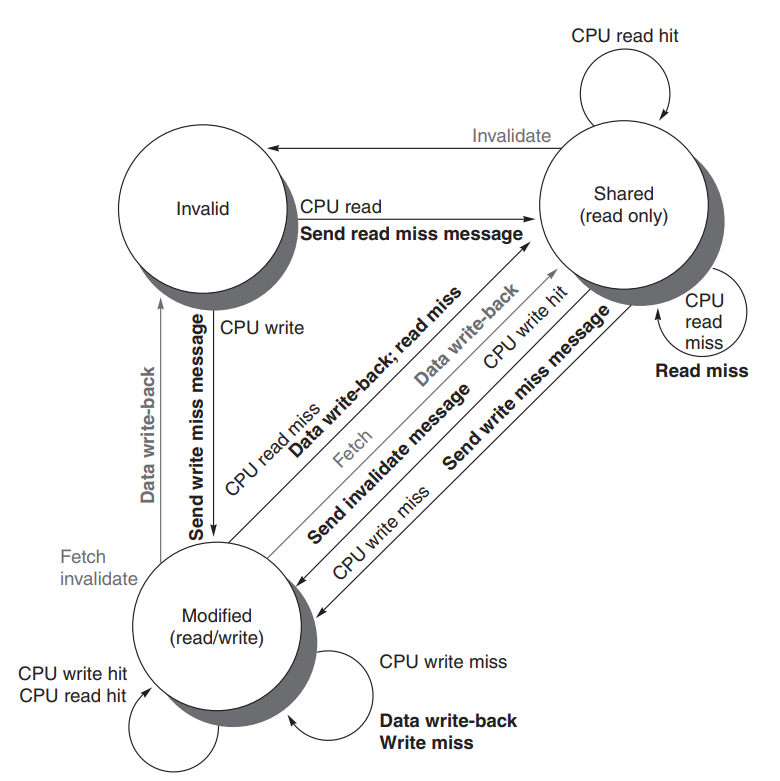
\includegraphics[width=0.8\textwidth, keepaspectratio]{imgs/directory-ts.png}
\caption{State transition diagram for an individual cache block in a directory-based system.}
\end{figure}
\section{Parallelisation}

\section{Program Transformations}

\end{document}
